%%\documentclass[12pt,letterpaper,doublespaced,ETD,dvips]{gt-ece-thesis}
\documentclass[12pt,letterpaper,doublespaced,ETD]{gt-ece-thesis} %taking dvips out enable pdf bookmark generation as well as the logo printing on the first page

\title{Target Tracking Using Residual Vector Quantization}
\author{Salman Aslam}
\copyrightyear{2011}
\graddate{20 June 2011}  
\approvaldate{June 2011}  

\addadvisor{Dr. Christopher F. Barnes}{Assoc. Professor, School of ECE}{Georgia Institute of Technology}
\addchair{Dr. David V. Anderson}{Assoc. Professor, School of ECE}{Georgia Institute of Technology}
\addreader{Dr. Aaron F. Bobick, Co-advisor}{Professor, School of Interactive Computing}{Georgia Institute of Technology}
\addreader{Dr. Vijay Madisetti}{Professor, School of ECE}{Georgia Institute of Technology}
\addreader{Dr. Patricio Vela}{Asst. Professor, School of ECE}{Georgia Institute of Technology}
\addreader{Dr. Santanu Dey}{Asst. Professor, School of ISYE}{Georgia Institute of Technology}


\bibfiles{f:/salman/work/writing/MyCitations}

\titlepagetrue
\figurespagetrue
\tablespagetrue
\contentspagetrue
\symbolspagefalse
\glossarypagefalse 
\bibpagetrue
\mastersthesisfalse 
\multivolumefalse
\singlespacednotestrue


\usepackage{graphicx, subfigure, verbatim}
\usepackage{insfig}
\usepackage{url}
\usepackage{multirow}
\usepackage{hyperref}
\usepackage{longtable}
\usepackage[usenames,dvipsnames]{color}
\definecolor{light-gray}{gray}{0.95}
\usepackage{amsmath,epsfig,verbatim,listings}
\lstset{breaklines=true,breakindent=0pt,
        prebreak=\mbox{\tiny$\searrow$},
        postbreak=\mbox{{\color{blue}\tiny$\rightarrow$}},
	tabsize=2,
linewidth=1.1\linewidth,
xleftmargin=-0.8in,
basicstyle=\tiny,
numbers=left,
frame=single,
captionpos=t,
title=\lstname,
backgroundcolor=\color{light-gray}}


\setchaptertocdepth{2}
\setappendixtocdepth{2}

\settocstring{Table of Contents}
\setlofstring{List of Figures}
%\setlotstring{List of Tables}
\setbibstring{References}
\setindstring{Index}
\setdedstring{Dedication}
\setglostring{List of Terms}
\setchpstring{Chapter}
\setappstring{Appendix}
\setprtstring{Volume}
\setabsstring{Summary}
\setlosstring{List of Symbols}
\setackstring{Acknowledgment}

\setfrontpagestyle{plain}
\setbodypagestyle{plain}
\setendpagestyle{plain}

\pagestyle{plain}
\bibliographystyle{ieeetr}
%\definecolor{darkgreen}{rgb}{0,0.5,0}
\newcommand{\Ntrg}{\big[N_{t=1, m=1} + \lambda \big] + \big[N_{t=1, m=2} + \lambda \big] + \ldots + \big[N_{t=1, m=M} + \lambda \big]}
\newcommand{\jointcnt}{\sum\limits_{n_{trg}=1}^{N_{trg}}I(X_t=x_t, X_{t-1}=x_{t-1})}
\newcommand{\singlecnt}{\sum\limits_{n_{trg}=1}^{N_{trg}}I(X_{t-1}=x_{t-1})}
\newcommand{\singlep}{p(X_{t-1}=x_{t-1})}
\newcommand{\singlepone}{p(X_{t-1}=1)}
\newcommand{\singleptwo}{p(X_{t-1}=2)}
\newcommand{\singlepM}{p(X_{t-1}=M)}
\newcommand{\condp}{p(X_t=x_t | X_{t-1}=x_{t-1})}
\newcommand{\jointp}{p(X_t=x_t, X_{t-1}=x_{t-1})}
\newcommand{\KmeansOuterSum}{\sum\limits_{k=1}^K}
\newcommand{\KmeansInnerSum}{\sum\limits_{{i=1 \atop x_i \in \mathcal{K}_k}}^N}
\newcommand{\KmeansSum}{\KmeansOuterSum \KmeansInnerSum}
\newcommand{\RVQInnerSum}{\sum\limits_{{i=1 \atop g_i \mapsto m_{\tau, s}}}^N}
\newcommand{\RVQOuterSum}{\sum_{s=1}^S}
\newcommand{\RVQsum}{\KmeansOuterSum \sum\limits_{{i=1 \atop g_i \in \mathcal{K}_k}}^N}
\newcommand{\KmeansInner}{{(x_i - \mu_k)}^2}
\newcommand{\RVQinner}{            {(x_i  - \hat{\mu}^{(k)})}^2}
\newcommand{\RVQinneralternate}{{(g_i - m_\tau^{(k)})}^2}
\newcommand{\RVQinneralternatealternate}{{(g_i - m_{\tau, s})}^2}
\newcommand{\KmeansError}{\KmeansSum \KmeansInner}
\newcommand{\RVQerror}     {\KmeansSum \RVQinner}
\newcommand{\RVQerroralternate}{\RVQsum \RVQinneralternate}
\newcommand{\RVQunit}{x_i -\bigg(\sum_{t=1}^Tm^{(k)}_t\bigg)}
\newcommand{\RVQequivalentCodevector}{\sum_{t=1 }^Tm^{(k)}_t}
\newcommand{\RVQequivalentCodevectorBroken}{\sum_{t=1 \atop t \neq \tau}^Tm^{(k)}_t+ m^{(k)}_\tau}
\newcommand{\RVQmultipleKmeans}{x_i -\bigg(\RVQequivalentCodevectorBroken\bigg)}
\newcommand{\RVQmultipleKmeansone}{x_i -\sum_{t=2}^Tm^{(k)}_t+ m^{(k)}_1\bigg)}
\newcommand{\RVQmultipleKmeansonealternate}{\bigg(x_i -\sum_{t=1 \atop t \neq \tau}^Tm^{(k)}_t\bigg) - m^{(k)}_\tau}
\newcommand{\RVQmultipleKmeanstwo}{x_i -\bigg(\sum_{t=1 \atop t \neq 2}^Tm^{(k)}_t+ m^{(k)}_2\bigg)}
\newcommand{\RVQmultipleKmeansT}{x_i -\bigg(\sum_{t=1}^{T-1}m^{(k)}_t+ m^{(k)}_2\bigg)}
\newcommand{\EucMatrix}
{
\left[
\begin{array}{lll}
r_{11} & r_{12} & t_x \\ 
r_{21} & r_{22} & t_y \\ 
0 & 0 & 1 \\ 
\end{array}
\right]
}	

\newcommand{\SimMatrix}
{
\left[
\begin{array}{lll}
sr_{11} & sr_{12} & t_x \\ 
sr_{21} & sr_{22} & t_y \\
0 & 0 & 1 \\ 
\end{array}
\right]
}

\newcommand{\AffMatrix}
{
\left[
\begin{array}{lll}
a &b & t_x \\ 
c & d & t_y \\
0 & 0 & 1 \\
\end{array}
\right]
}

\newcommand{\ProjMatrix}
{
\left[
\begin{array}{lll}
h_{11} & h_{12} & h_{13} \\ 
h_{21} & h_{22} & h_{23} \\ 
h_{31} & h_{32} & h_{33} \\ 
\end{array}
\right]
}

\newcommand{\RotMatrixTheta}
{
\left[
\begin{array}{rr}
\cos(\theta) & -\sin(\theta) \\ 
\sin(\theta) & \cos(\theta) \\ 
\end{array}
\right]
}

\newcommand{\RotMatrixPhi}
{
\left[
\begin{array}{rr}
\cos(\phi) & -\sin(\phi) \\ 
\sin(\phi) & \cos(\phi) \\ 
\end{array}
\right]
}

\newcommand{\RotMatrixminusPhi}
{
\left[
\begin{array}{rr}
\cos(-\phi) & -\sin(-\phi) \\ 
\sin(-\phi) & \cos(-\phi) \\ 
\end{array}
\right]
}


\newcommand{\EigenvalueMatrix}
{
\left[
\begin{array}{cc}
\lambda_1 & 0\\
0 & \lambda_2
\end{array}
\right]
}

\newcommand{\bigMatrix}
{
s \left[
\begin{array}{cc}
 (r)(a) + b &  (r)(d) - c \\
 (r)(c) - d &  (r)(b) + a
\end{array}
\right]
}


\newcommand{\bigMatrixTwo}
{
\left[
\begin{array}{cc}
(\lambda_2) p + (\lambda_1) q & (\lambda_2) s  - (\lambda_1) r \\
(\lambda_2) r  - (\lambda_1) s & (\lambda_2) q + (\lambda_1) p
\end{array}
\right]
}
\newcommand{\dr}{(\mathbf{x}_i-\boldsymbol\mu_k)^T(\mathbf{x}_i-\boldsymbol\mu_k) + \lambda({Q_{\textrm{max}}-Q_i})}

%\begin{document}
%\begin{FrontMatter}
%\contents %generates the TOC, LOF, and LOT
%\end{FrontMatter}
%\begin{Body}

%@@@@@@@@@@@@@@@@@@@@@@@@@@@@@@@@@@@@@@@@@@@@@@@@@@
\chapter{Visual Tracking Using RVQ}
\label{chap_RVQ_TRK}	
%@@@@@@@@@@@@@@@@@@@@@@@@@@@@@@@@@@@@@@@@@@@@@@@@@@
%===================
\section{Introduction}
%===================
In this chapter, we combine information on target representations presented in Chapter~\ref{chap_Introduction}, theoretical knowledge of RVQ presented in Chaper~\ref{chap_RVQ} and an overview of tracking methods presented in Chapter~\ref{chap_TRK} into a visual tracking framework using RVQ and compare it with visual tracking using PCA and TSVQ.  

This work is significant since PCA is commonly used in the Pattern Recognition, Machine Learning and Computer Vision communities.  On the other hand, TSVQ is commonly used in the Signal Processing and data compression communities.  RVQ with more than two stages has not received much attention due to the difficulty in producing stable designs.  In this work, we bring together these different approaches and compare them in a combined visual tracking framework.  The result is a robust tracker for all 3 methods, but with RVQ performing the best according to certain defined criteria to be described later in the chapter.  Moreover, an advantage of our approach is a learning-based tracking framework that builds the target model while it tracks, thus avoiding the costly step of building target models prior to tracking~\cite{2004_JNL_SVMtracking_Avidan}.

The approach we take in this work builds on work presented by Ross et. al. in 2008 \cite{2008_JNL_subspaceTRK_Ross}.  As a matter of fact, we have used part of their software with their permission~\cite{2008_SFT_Ross}.  In this spirit, we make our software available for download to the community at \url{https://github.com/SalmanAslamPhD/PhD}.  

%----------------------------------------
\subsection{Challenges}
%----------------------------------------
Visual tracking is the task of estimating a target's state over time.  In many cases, the state represents target position and a bounding box, or its contour.  This is a challenging problem due to the following reasons:

\begin{enumerate}
\item \underline{Appearance and contour changes}:  A target of interest can undergo arbitrary change in appearance and contour.  This can be due to the following reasons:
\begin{enumerate}
\item \underline{Pose change}:  The target can rotate and present a different view to the camera.
\item \underline{Warping}: The target can undergo warps, such as expression changes for humans.
\item \underline{Self occlusion}:  The target can be occluded or unoccluded by itself or its surroundings.
\item \underline{Blur}:  Motion blur can severely distort a target's appearance.
\item \underline{Structured noise}:  The target can change appearance in an orderly manner, for instance, a target of interest can put on or remove glasses or a hat.
\item \underline{Random noise}:  This can be a result of atmospheric effects in the optical channel, sensor noise, electronics noise and EMI (electromagnetic interference).  On the software side, it can be caused by compression artefacts.
\item \underline{Non-symmetic BRDF}:  The light reflected off of an object in all directions is modeled by the bidirectional radiation transfer function (BRDF)\footnote{BRDF is given by $\rho(\theta_o, \phi_o, \theta_i, \phi_i)=\frac{L_o(x, \theta_o, \phi_o)}{L_i(x, \theta_i, \phi_i)\cos\theta_i d\omega}$, where the angles ($\theta_o, \phi_o$) define the outgoing light direction and angles ($\theta_i, \phi_i$) define the incoming light direction.  A surface illuminated by radiance $L_i(x, \theta_i, \phi_i)$ coming in from a differential region of solid angle $d\omega$ at angles $\theta_i, \phi_i$ receives irradiance $L_i(x, \theta_i, \phi_i)\cos\theta_i d\omega$.  Irradiance is measured in $\mathrm{W/m^2}$, while the solid angle $d\omega$ is measured in steridians, sr.  The unit of BRDF is therefore $\mathrm{sr^{-1}}$~\cite{2002_BOOK_CV_Forsyth}.}.  Since this function may not be symmetric in all directions, the amount of light reflecting off of the object may be different in different directions.  Multiple cameras viewing the same point will receive different intensity levels.
\end{enumerate}
\item \underline{Lighting change}: Lighting changes can be caused by turning on or off lights in indoor environments, or moving into or out of shades in outdoor environments.
\item \underline{Sudden motion (target or camera)}:  Besides motion blur, sudden motion by the target or camera can cause the target to exit the window in which the tracker looks for the target leading to incorrect track assignment.
\end{enumerate}

For a tracker that tries to learn the appearance and/or contour model of the target, inclusion of background pixels is an added problem that can cause drift.  If none of the problems mentioned above were present, a simple template matching stategy would suffice for robust tracking.  This has complexity $O(nm)$, where $n$ is the number of pixels in the target and $m$ is the number of locations at which the target is searched.  For most practical situations, this does not represent significant computational load and can be done in real time even while tracking several targets.  However, in the presence of several forms of noise, which is generally the case in tracking applications, more sophisticated methods are required.  In this chapter, we focus on methods involving compact representations of the target appearance model, i.e., PCA, TSVQ and RVQ.



%----------------------------------------
\subsection{Brief history}
%----------------------------------------
								\begin{figure}[t]
								\centering
								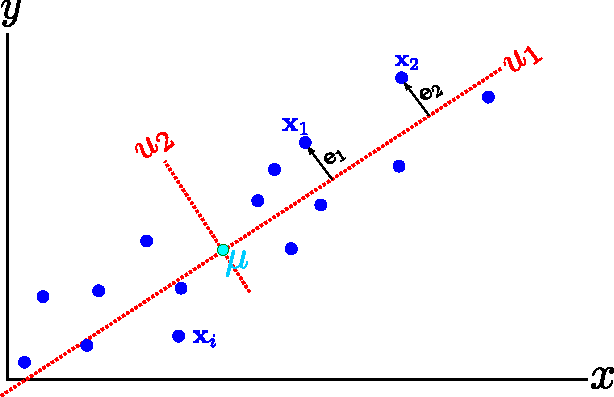
\includegraphics[width=0.45\textwidth]{thesis/PRML_PCA_problem.pdf}
								\caption{In $\mathbb{R}^2$, a reduced eigenspace means that eigenvector $u_2$ is discarded.  Vectors $\mathbf{x}_1$ and $\mathbf{x}_2$ have the same projection error on eigenvector $u_1$ even though $\mathbf{x}_1$ is closer to the mean $\boldsymbol\mu$ of the training data $\mathbf{x}_i$.}
								\label{fig:PRML_PCA_problem}
								\end{figure}

								\begin{figure}[t]
								\centering
								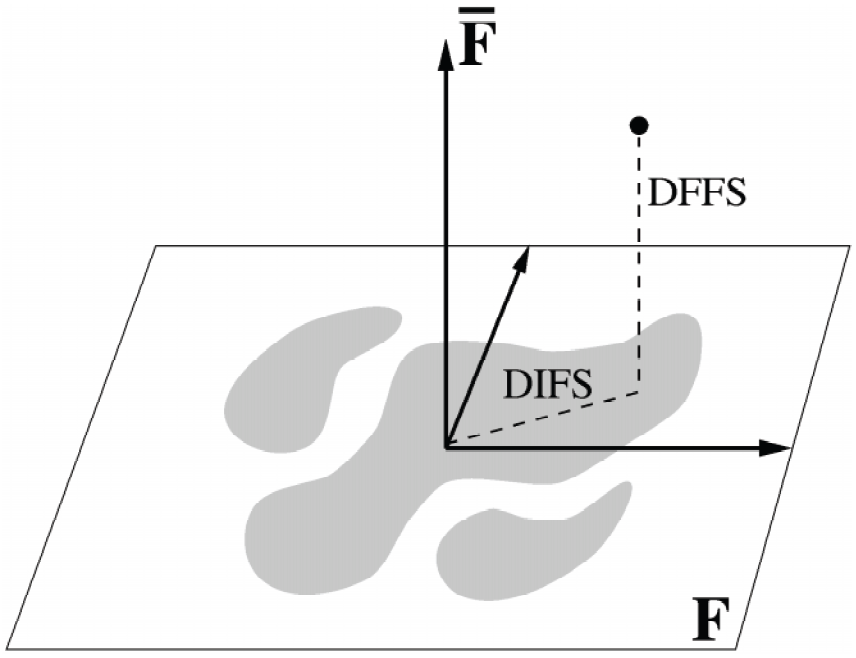
\includegraphics[width=0.5\textwidth]{thesis/1998_JNL_ProbVisLearning_Moghaddam_fig3.png}
								\caption{Graphical illustration of DFFS (distance-from-feature-space) and DIFS (distance-in-feature-space).  The feature space is $\mathbf{F}$ while the subspace orthogonal to the feature space is $\bar{\mathbf{F}}$.  DFFS is the signal residual error and DIFS is the $\mathbf{F}$-space likelihood \cite{1997_JNL_EigenTRK_Moghaddam}.}
					\label{fig:1997_JNL_DIFSDFFS_Moghaddam}
								\end{figure}

In this work, we try to address single-target visual-tracking under several of the challenges mentioned above while trying to learn the appearance model of the target.  Seminal work here can be traced back to 1996 when Black and Jepson experimented with tracking using an eigenspace representation of the target appearance model~\cite{1998_JNL_Eigentracking_Black}.  The next notable work is by Moghaddam and Pentland, 1997~\cite{1997_JNL_EigenTRK_Moghaddam} in which they try to address a fundamental limitation of PCA.  In PCA, 2 vectors, $\mathbf{x}_1$ and $\mathbf{x}_2$ can have the same distance to a reduced eigenspace, i.e., projection error $\mathbf{e}_1$ and $\mathbf{e}_2$ respectively, even if they have different distance to the mean $\boldsymbol\mu$ of the data that was used to create the eigenspace.  This is shown for a trivial case in $\mathbb{R}^2$ in Figure~\ref{fig:PRML_PCA_problem} where $\mathbf{e}_1=\mathbf{e}_2=\mathbf{e}$ even though $\mathbf{x}_1$ is closer than $\mathbf{x}_2$ to the mean $\boldsymbol\mu$.  They formulate the problem using DIFS (distance in feature space) and DFFS (distance from feature space) so that both projection error and within-subspace distance to the mean of the data are used while trying to determine how well the subspace explains a new data-point.  The next breakthrough came with the work of Bishop and Tipping in 1999~\cite{1999_JNL_PPCA_Tipping} where they show that a probabilistic variation of PCA, probabilistic PCA (PPCA), allows PCA to be used as a generative model.  The advantage in tracking is that this methodology allows an assignment of probabilities to new data-points and therefore allows relative weighting of track candidates.  Ideas from these three works were combined into a tracking framework by Ross et. al. in 2008~\cite{2008_JNL_subspaceTRK_Ross}.  Moreover, they used incremental SVD to make their tracker run in real time.  

Here, we extend the work in Ross et. al.~\cite{2008_JNL_subspaceTRK_Ross} using RVQ in a similar tracking framework and comparing it with PCA and TSVQ based tracking.  We also introduce 4 methods for relative weighting of track candidates for RVQ.  The result is a generative framework for RVQ that leads to robust tracking.  Whereas RVQ was first introduced by Juang and Gray in 1982~\cite{1982_CNF_SpeechRVQ_JuangGray} and subsequently greatly extended by the seminal work of Barnes~\cite{1991_CNF_DesignPerformanceRVQ_Frost,1992_JNL_RVQ_Barnes,1992_CNF_ImageCodingRVQ_Kossentini,1993_sigmaTrees_Barnes,1993_JNL_RVQDSC_Barnes,1995_JNL_OptimalityRVQ_Kossentini,1996_CNF_VQclassification_Barnes,1996_JNL_AdvancesRVQ_Barnes,2002_JNL_SigmaTrees_Barnes,2004_CNF_DSSAdataMining_Barnes,2007_JNL_Katrina_Barnes,2007_JNL_IDDM_Barnes}, this algorithm has received little attention outside the signal processing and data compression communities.  In this work our goal is to introduce RVQ in the computer vision and machine learning fields where a much simpler version, K-means, has been widely used~\cite{2008_JNL_PRML_Wu}.  We present RVQ in the context of an important and challenging problem, that of visual target tracking.

%----------------------------------------------------
\subsection{Overview of approach used}
%----------------------------------------------------
								\begin{figure}[t]
								\centering
								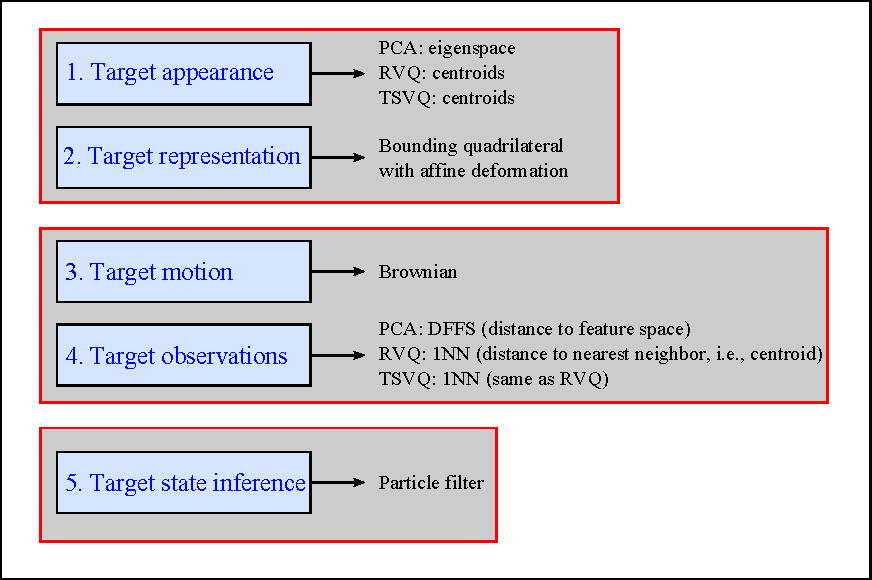
\includegraphics[width=1.0\textwidth]{thesis/PhD_experimentalOverview.pdf}
								\caption{Tracking framework, overview.}
								\label{fig:overview}
								\end{figure}

Our goal is to produce estimates at every time frame of the target state, i.e. 6 affine parameters that define a target bounding quad.  In order to accomplish this, our tracking framework is based on five components as shown in Figure~\ref{fig:overview} .  Each of these components is described in detail in later sections.  Here, we present an overview of each:

\begin{enumerate}
\item \underline{Appearance model}.  The goal of the appearance model is to provide a compact representation of the target's pixel intensities.  In this work, we use a learned eigenspace, a trained $\sigma$-tree codebook or a binary balanced-tree codebook for PCA, RVQ and TSVQ respectively.  Refer to Chapter~\ref{chap_RVQ} for a description of RVQ.

\item \underline{Observation model}.  The goal of the observation model is to generate a likelihood score for an observation.  For PCA, the likelihood of a target observation is assumed proportional to the DFFS (distance to feature space).  For RVQ, the likelihood of a target observation is assumed to be proportional to the Euclidean distance to the closest equivalent code-vector, as explained in Chapter~\ref{chap_RVQ}, or partially summed code-vector as explained later in this chapter.  We use 2 methods, maxP and RofE, to compute the equivalent code-vector, and 2 methods, nulE and monR to compute the partially summed code-vector.  These methods are also explained later in this chapter. For TSVQ, the likelihood of a target observation is assumed to be proportional to the Euclidean distance to the closest terminal code-vector.

\item \underline{Representation model}.  The goal of the representation model is to provide a means of specifying a target.  Several target representation methods are described in Chapter~\ref{chap_Introduction}.  We use the bounding quadrilateral method.  This quad encloses the pixels of a target of interest.  It is also allowed to warp affinely from frame to frame to minimize inclusion of background pixels as the target changes shape, size and orientation.

\item \underline{Motion  model}.  The goal of the motion model is to specify the motion that the target is expected to follow.  In order to keep our work general, we do not assume any deterministic target motion model.  The target is expected to move according to a Wiener process, i.e., brownian motion.  This allows for robust tracking under arbitrary target and camera motion.

\item \underline{Inference model}.  The goal of the inference model is to: (a) weight the likelihoods of various observations and make a decision on which observation should be picked as an estimate for the target position and appearance, and (b) keep a temporal record of which observations were not picked in the previous frames as best estimates but may still potentially be considered in future frames.  In tracking, the correspondence of observations in the current frame to existing targets in the previous frame is generally an ill-posed problem~\cite{2005_CNF_TRK_Yang}.  We use the particle filter to deal with this problem by propagating multiple hypotheses from frame to frame~\cite{1998_JNL_Condensation_IsardBlake}.  The computational complexity of this method does not grow with frames as opposed to the multi-hypothesis tracker (MHT)~\cite{1993_JNL_SURVEYcorresp_Cox}.
\end{enumerate}

These models work together to produce state estimates at every time frame.  The motion model and the representation model work together to generate 600 affine parameter sets as candidates for the target state.  The observation model takes these affine parameter sets and extracts observations, i.e., candidate window-chips, also called \emph{snippets}~\cite{2007_JNL_IDDM_Barnes} from the image.  It then uses the appearance model to generate a likelihood score for each snippet.  Finally, the inference model picks the snippet with the highest score and goes through a resampling step so that snippets with low likelihood scores are eliminated and snippets with high likelihood scores are repeated.  The affine parameters of these resampled snippets are then given to the motion model in the next frame and the process continues.

%----------------------------------------------
\subsection{Overview of temporal process}
%----------------------------------------------
								\begin{figure}[t]
								\centering
								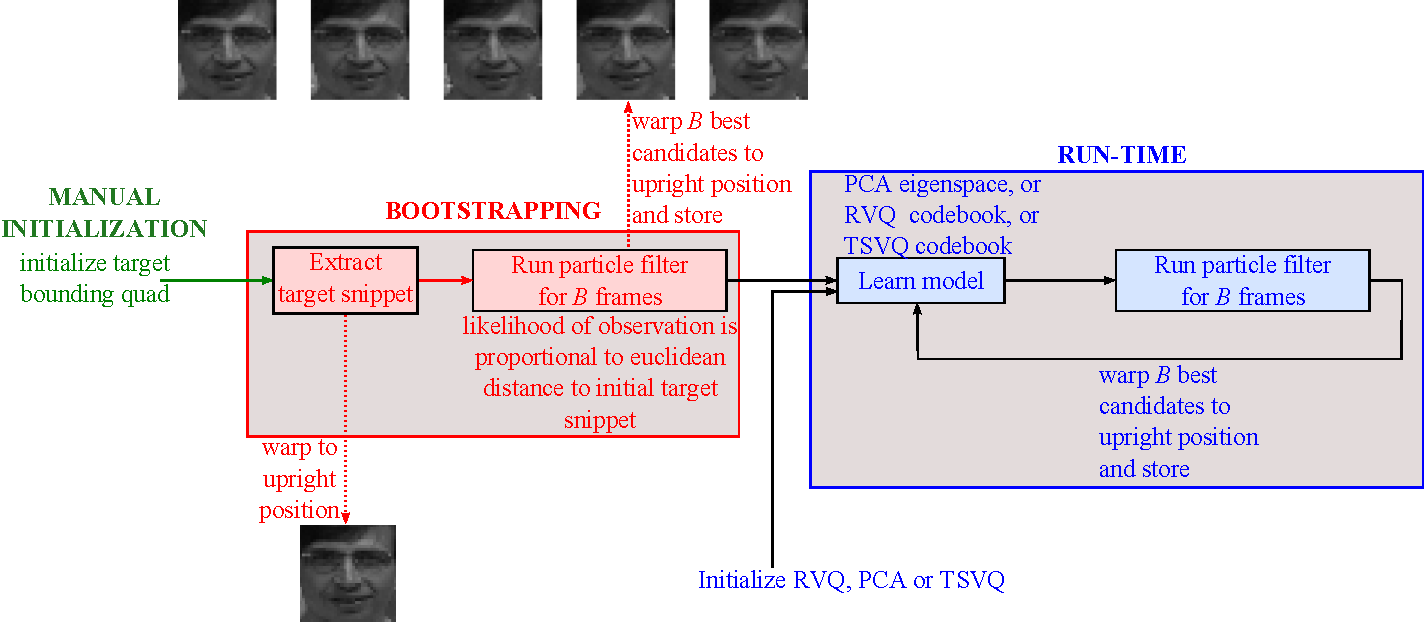
\includegraphics[width=1.1\textwidth]{thesis/PhD_experimentalTemporalOverview.pdf}
								\caption{Temporal overview.}
								\label{fig:temporal_overview}
								\end{figure}

In the previous section, we described the five major components of our visual tracking framework and their mutual interaction.  In this section, we describe the temporal evolution of the tracking process.  Refer to Figure~\ref{fig:temporal_overview} for a graphical overview.  The temporal process is based on 3 distinct phases:

\begin{enumerate}
\item \underline{Manual initialization}.  The target is identified in the first frame by manually drawing a bounding box around it and identifying certain feature points on it.  For instance, for the Dudek sequence in which a face is tracked, feature points include the outer edges of the eye and points on the lips.  For the car11 sequence in which a car is tracked from the read, feature points include the tail lights.

%The box is allowed to be affinely deformed as discussed later in this chapter.  Template matching then allows a certain number of frames to be designated as initial training frames.  Currently this value is set to $N_B=5$. 

\item \underline{Bootstrapping}.  A particle filter is run for $B$ frames.  The likelihood of observations is computed using the Euclidean distance from the manually segmented target in the first frame.  The $B$ maximum aposteriori (MAP) snippets, one from each of the $B$ frames are stored.

\item \underline{Run-time}.  During this step, the learning process and the particle run alternately.  For PCA, the learning process includes updating its eigenbasis with the MAP estimates of the particle filter.  For RVQ and TSVQ, the learning process includes updating their codebooks. 
\end{enumerate}


%This model ties in multiple possible spatial observations in a temporal framework to enable sequential inference through the tracking process.
%Every frame after the one-time initialization is tested against the iPCA, bPCA, RVQ and TSVQ models and results are compared.  The Condensation algorithm is used for temporal and spatial integration of observation and state information.  Spatial processing includes generating several candidate window chips (snippets) and picking the one that gives least mean squared reconstruction error.  Temporal processing includes carrying over the posterior density from a frame as the prior density for the next frame.  The snippet that gives the least squared error is retained and added to the pool of training images in FIFO (first-in first-out) fashion, i.e. a moving window of $N_w$ training images is maintained.

Our tracking framework based on the 5 models mentioned in the previous section working through the temporal process explained in this section enable us to handle the following tracking challenges:

\begin{itemize}
\item \underline{Target appearance related}: Target pose changes, lighting changes, structured noise and temporary occlusions.
\item  \underline{Target representation related}: Target scale and orientation changes.
\item  \underline{Target motion related}: Arbitrary camera and target motion.
\end{itemize}

We now discuss each of the 5 models of our tracking framework (see Figure~\ref{fig:overview}).  

%============================
\section{Model 1: Appearance model}
\label{Sec:RVQ_trk_appearance_model}
%============================
								\begin{figure}[t]
								\subfigure[Uniform random variable $U\sim$ \texttt{[}0, 1\texttt{]} in $\mathbb{R}^{1089}$, 100 realizations.]{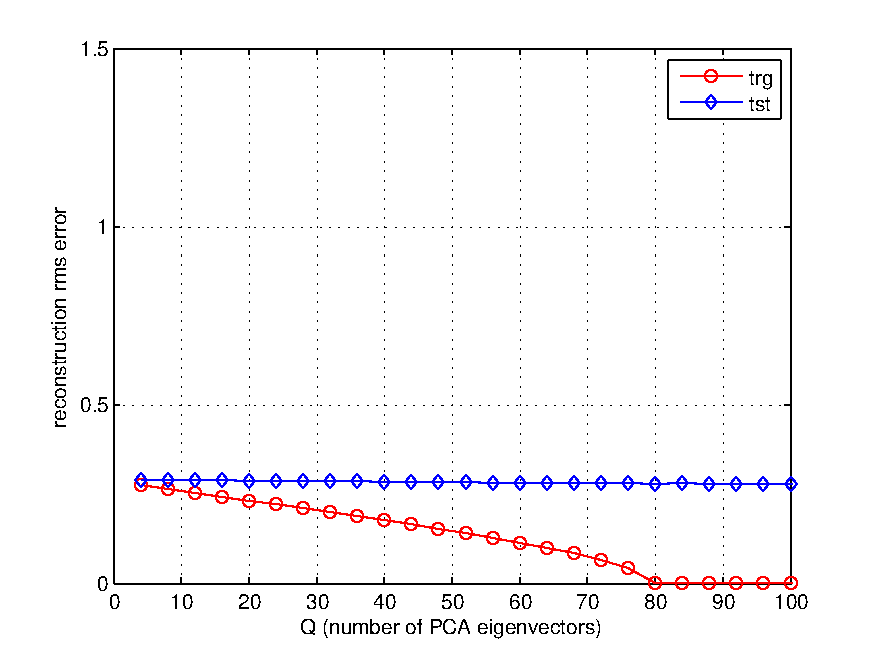
\includegraphics[width=0.45\textwidth]{thesis/PCA_Uniform.pdf}}
								\subfigure[Gaussian random variable $\mathcal{N}\sim$(0, 1) in $\mathbb{R}^{1089}$, 100 realizations.]{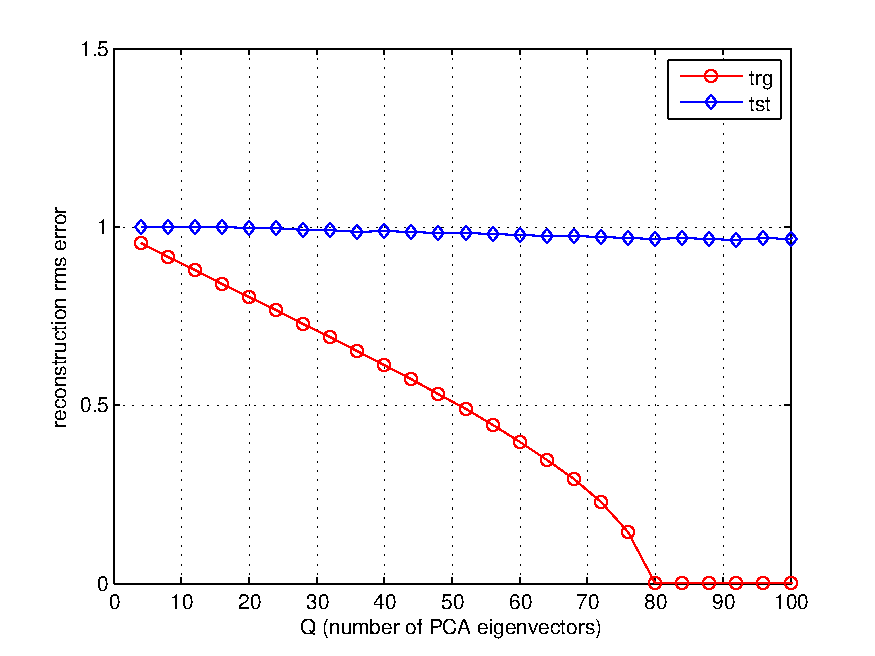
\includegraphics[width=0.45\textwidth]{thesis/PCA_Gaussian.pdf}}
								\subfigure[Gauss-Markov random variable $\mathcal{N}\sim$(0, 1) in $\mathbb{R}^{1089}$ with 0.9 correlation, 100 realizations.]{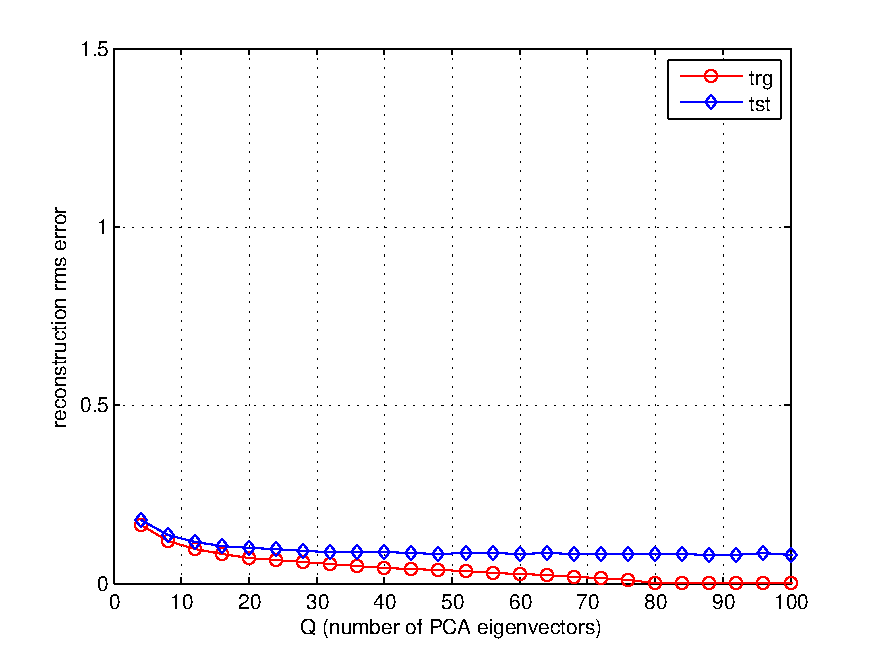
\includegraphics[width=0.45\textwidth]{thesis/PCA_GaussMarkov.pdf}}\hspace{0.55in}
								\subfigure[Dudek sequence, 33x33 ($\mathbb{R}^{1089}$) face snippets were extracted from the first 100 images.]{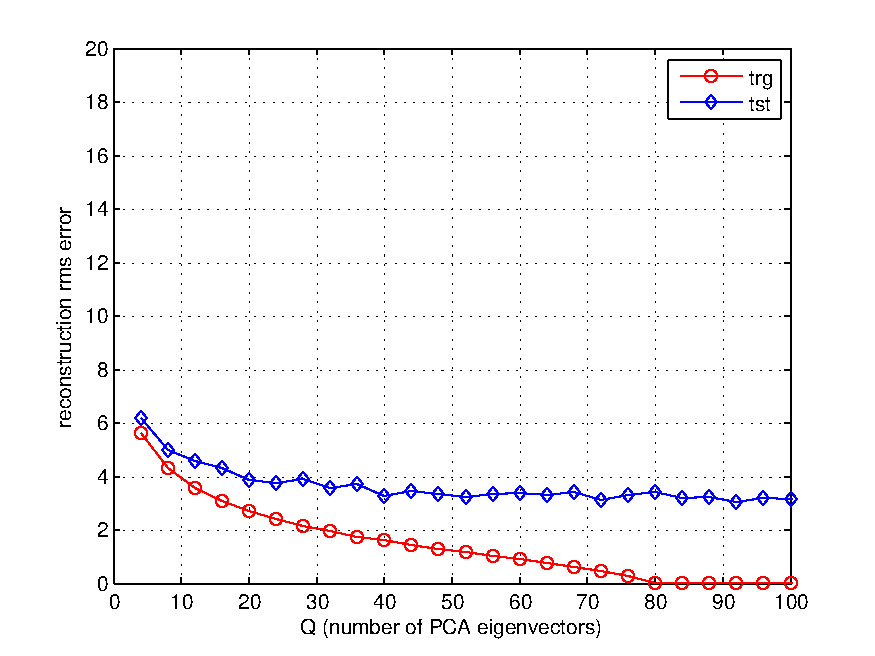
\includegraphics[width=0.45\textwidth]{thesis/PCA_Dudek.pdf}}
								\caption{PCA, 100 training examples in $\mathbb{R}^{1089}$ were used for each of these experiments. Results were averaged over 10 cross-validation runs. For each run, 20\% of the data, i.e., 20 examples were randomly picked for testing while the remaining 80 examples were used for training.}
								\label{fig:PCA_results}
								\end{figure}
								
								\begin{figure}[t]
								\subfigure[Uniform random variable $U\sim$ \texttt{[}0, 1\texttt{]} in $\mathbb{R}^{1089}$, 100 realizations.]
								{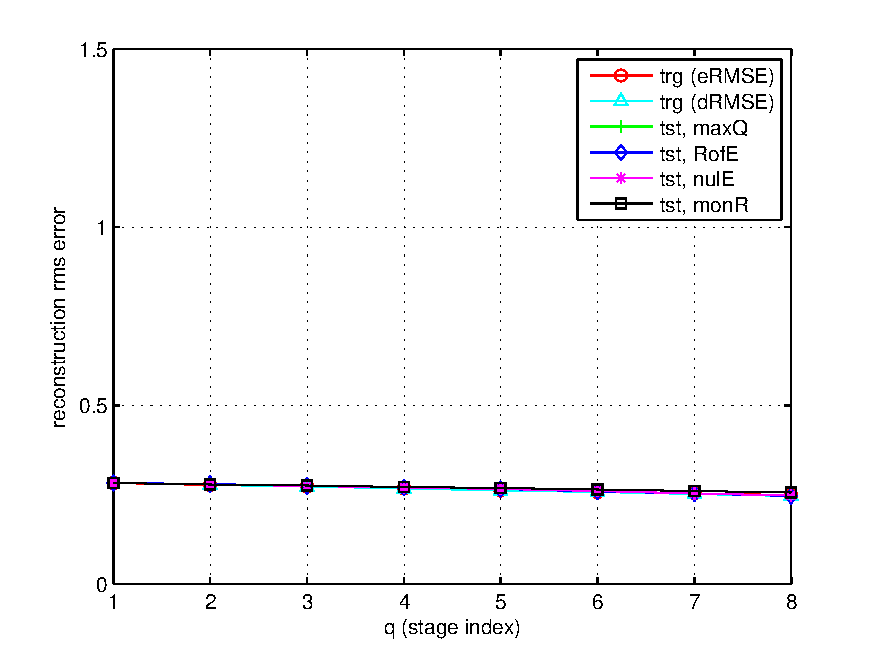
\includegraphics[width=0.45\textwidth]{thesis/RVQ_8x4_Uniform.pdf}}
								\subfigure[Gaussian random variable $\mathcal{N}\sim$(0, 1) in $\mathbb{R}^{1089}$, 100 realizations.]
								{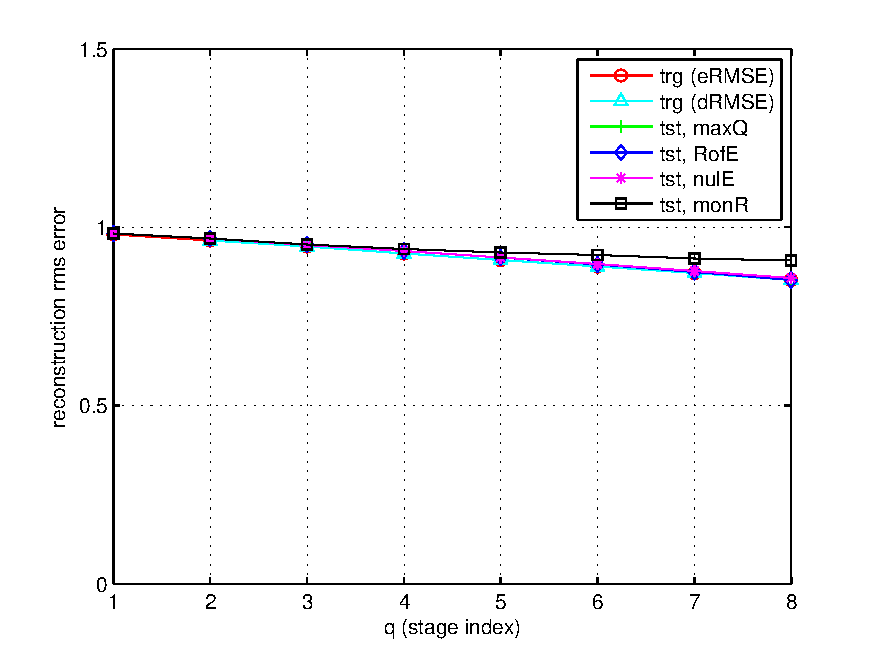
\includegraphics[width=0.45\textwidth]{thesis/RVQ_8x4_Gaussian.pdf}}
								\subfigure[Gauss-Markov random variable $\mathcal{N}\sim$(0, 1) in $\mathbb{R}^{1089}$ with 0.9 correlation, 100 realizations.]
								{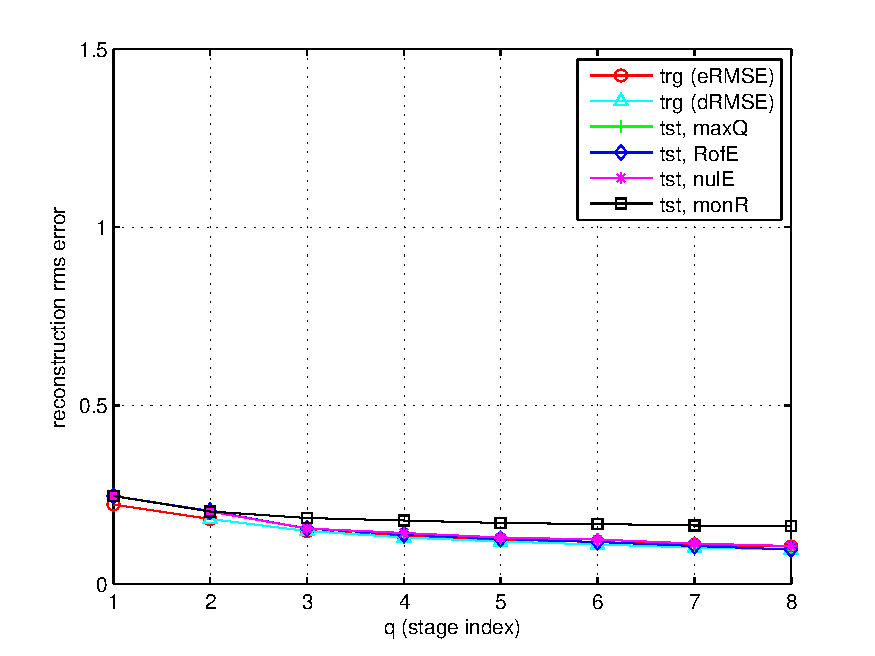
\includegraphics[width=0.45\textwidth]{thesis/RVQ_8x4_GaussMarkov.pdf}}\hspace{0.55in}
								\subfigure[Dudek sequence, 33x33 ($\mathbb{R}^{1089}$) face snippets were extracted from the first 100 images.]
								{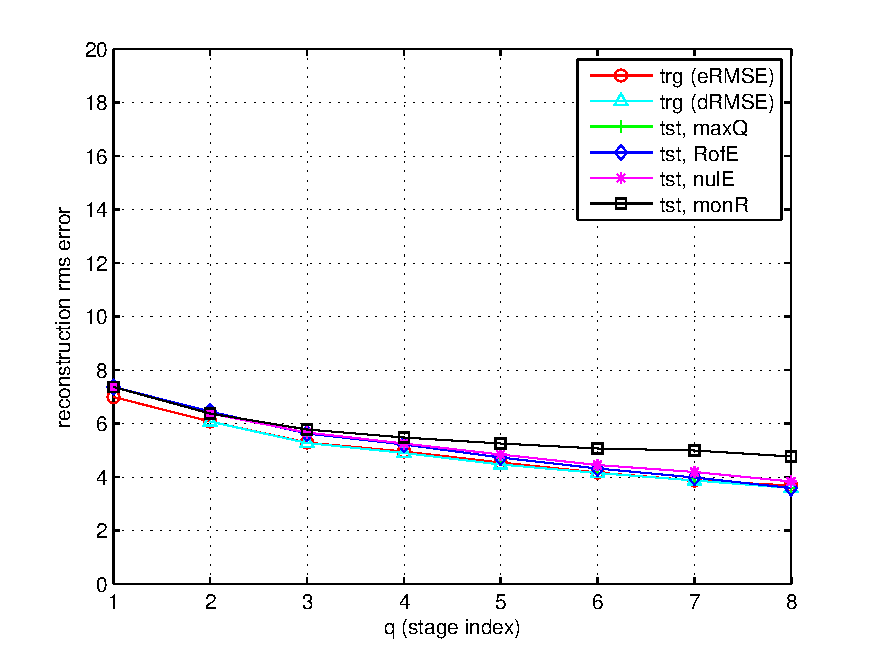
\includegraphics[width=0.45\textwidth]{thesis/RVQ_8x4_Dudek.pdf}}
								\caption{RVQp, varying number of stages $P$ with number of code-vectors per stage held constant at $M=4$. 100 training examples in $\mathbb{R}^{1089}$ were used for each of these experiments. A single test example in $\mathbb{R}^{1089}$ was reconstructed.}
								\label{fig:RVQ_results_varyingP}
								\end{figure}
								
								\begin{figure}[t]
								\subfigure[Uniform random variable $U\sim$ \texttt{[}0, 1\texttt{]} in $\mathbb{R}^{1089}$, 100 realizations.]
								{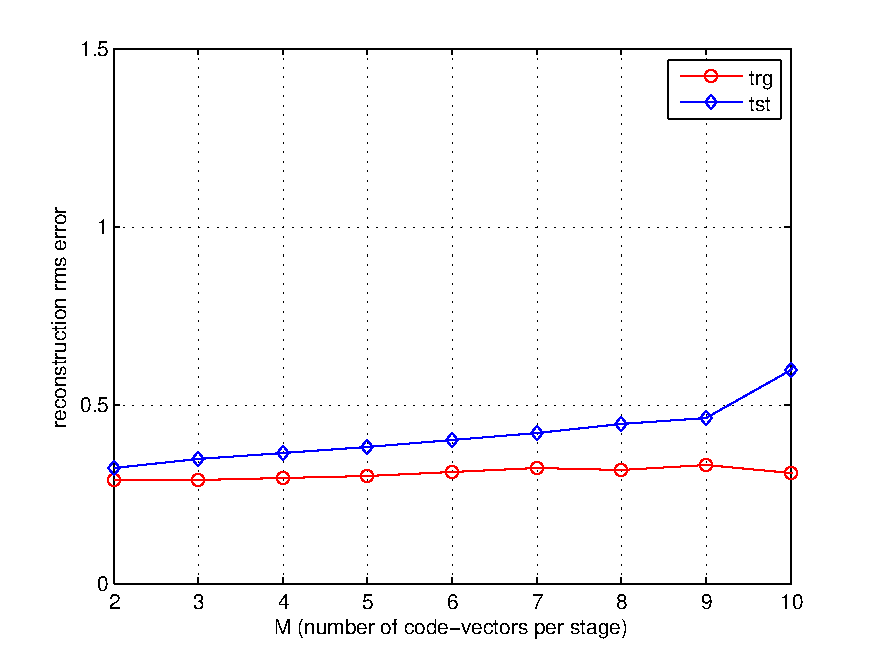
\includegraphics[width=0.45\textwidth]{thesis/RVQ_uniform.pdf}}
								\subfigure[Gaussian random variable $\mathcal{N}\sim$(0, 1) in $\mathbb{R}^{1089}$, 100 realizations.]
								{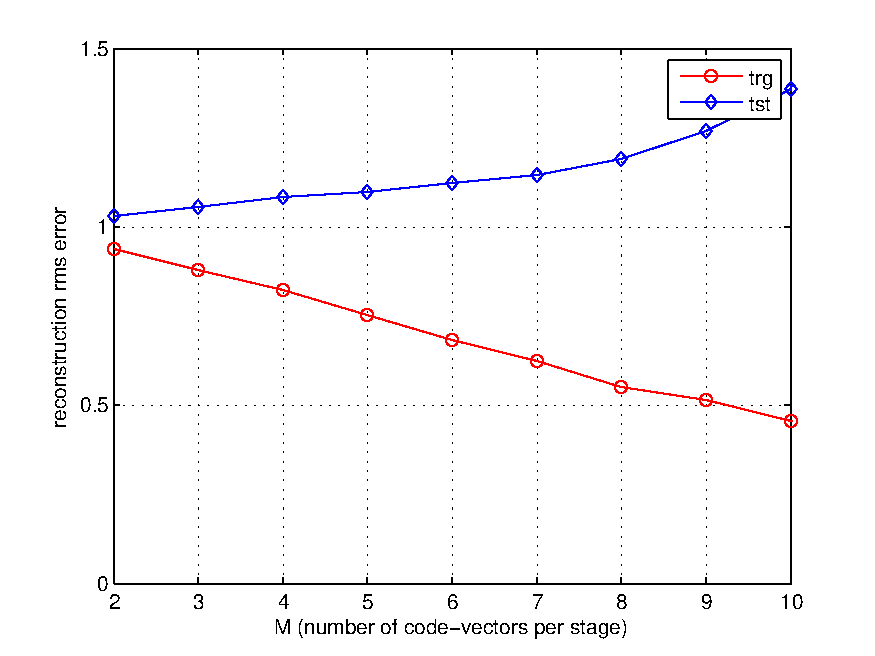
\includegraphics[width=0.45\textwidth]{thesis/RVQ_Gaussian.pdf}}
								\subfigure[Gauss-Markov random variable $\mathcal{N}\sim$(0, 1) in $\mathbb{R}^{1089}$ with 0.9 correlation, 100 realizations.]
								{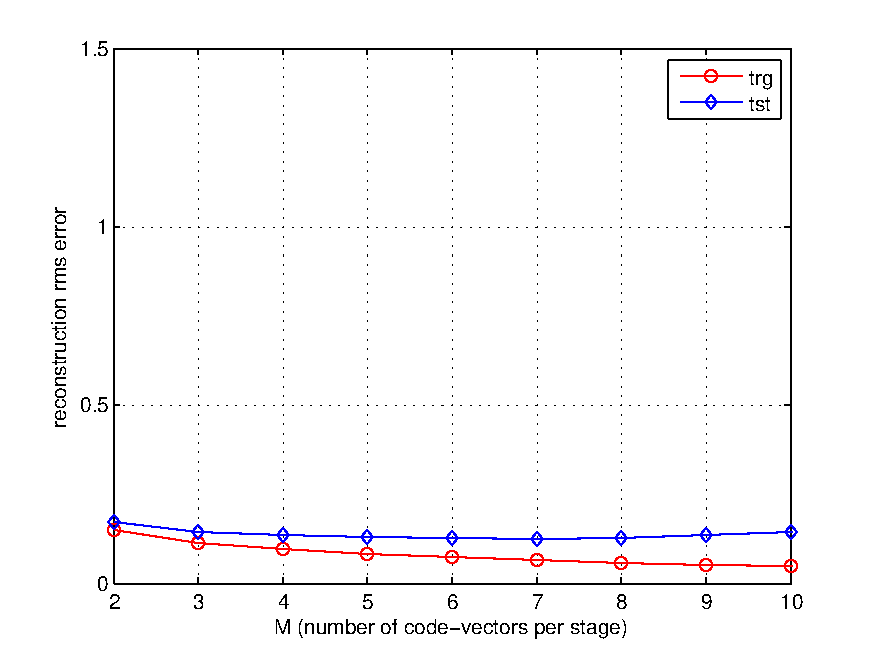
\includegraphics[width=0.45\textwidth]{thesis/RVQ_GaussMarkov.pdf}}\hspace{0.55in}
								\subfigure[Dudek sequence, 33x33 ($\mathbb{R}^{1089}$) face snippets were extracted from the first 100 images.]
								{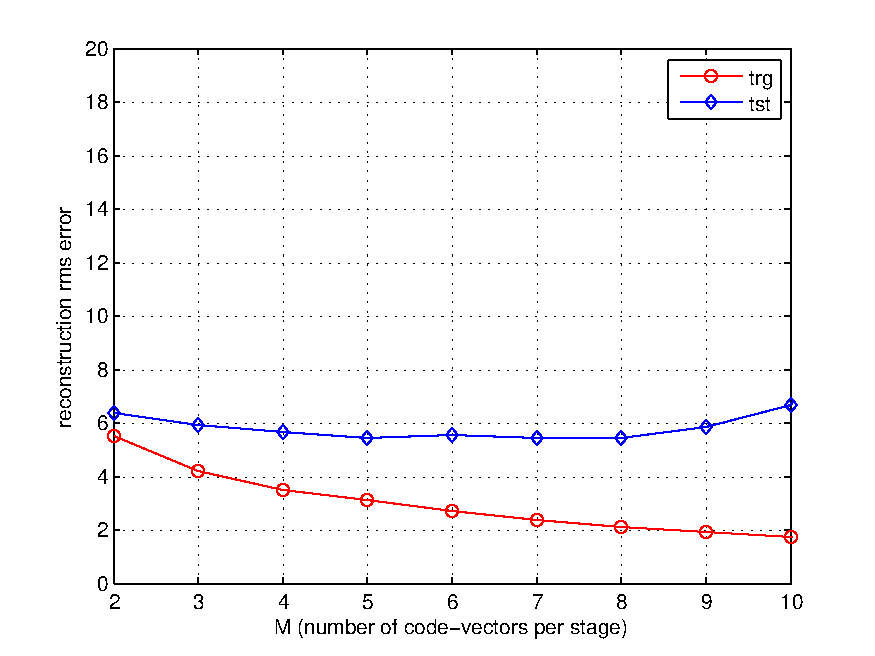
\includegraphics[width=0.45\textwidth]{thesis/RVQ_Dudek.pdf}}
								\caption{RVQm, experiments, varying number of code-vectors per stage $M$ with number of stages held constant at $P=8$. 100 training examples in $\mathbb{R}^{1089}$ were used for each of these experiments. Results were averaged over 10 cross-validation runs. For each run, 20\% of the data, i.e., 20 examples were randomly picked for testing while the remaining 80 examples were used for training.}
								\label{fig:RVQ_results_varyingM}
								\end{figure}
								
								\begin{figure}[t]
								\subfigure[Uniform random variable $U\sim$ \texttt{[}0, 1\texttt{]} in $\mathbb{R}^{1089}$, 100 realizations.]{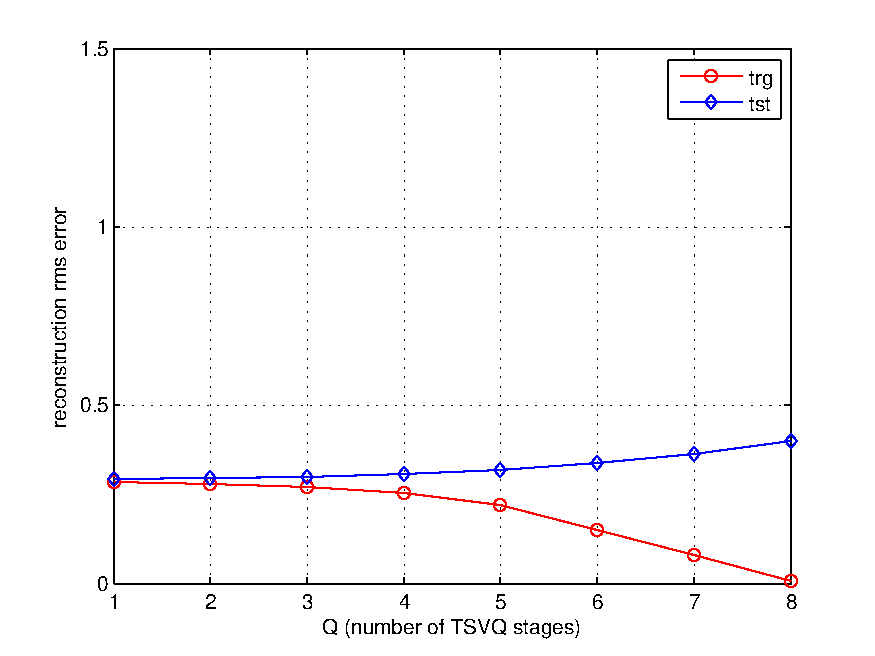
\includegraphics[width=0.45\textwidth]{thesis/TSVQ_Uniform.pdf}}
								\subfigure[Gaussian random variable $\mathcal{N}\sim$(0, 1) in $\mathbb{R}^{1089}$, 100 realizations.]{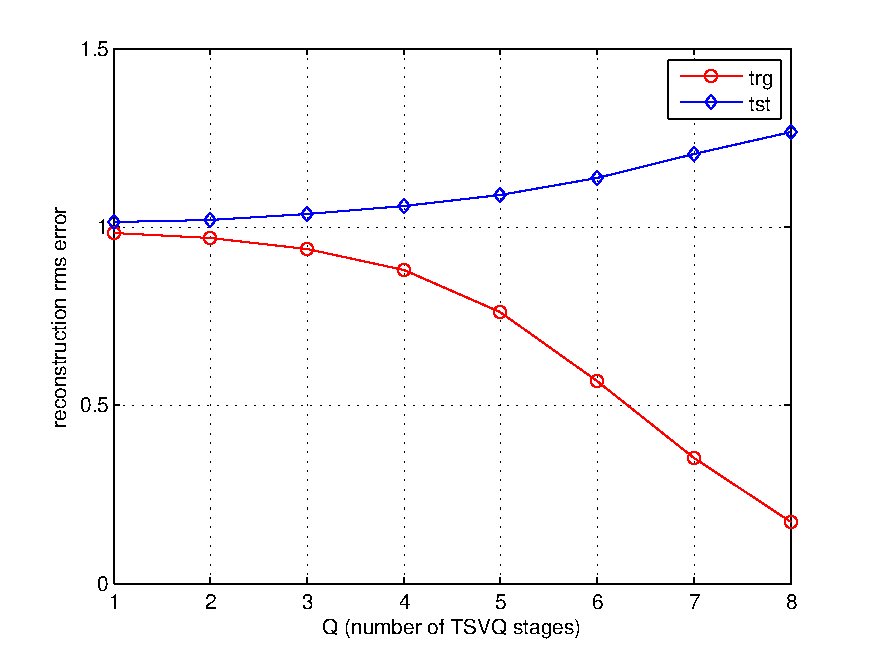
\includegraphics[width=0.45\textwidth]{thesis/TSVQ_Gaussian.pdf}}
								\subfigure[Gauss-Markov random variable $\mathcal{N}\sim$(0, 1) in $\mathbb{R}^{1089}$ with 0.9 correlation, 100 realizations.]{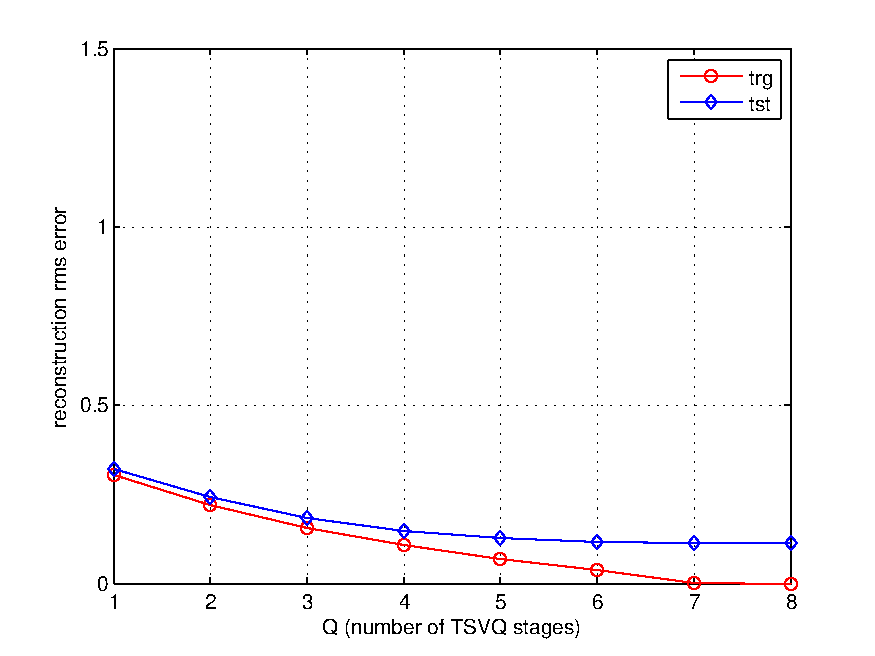
\includegraphics[width=0.45\textwidth]{thesis/TSVQ_GaussMarkov.pdf}}\hspace{0.55in}
								\subfigure[Dudek sequence, 33x33 ($\mathbb{R}^{1089}$) face snippets were extracted from the first 100 images.]{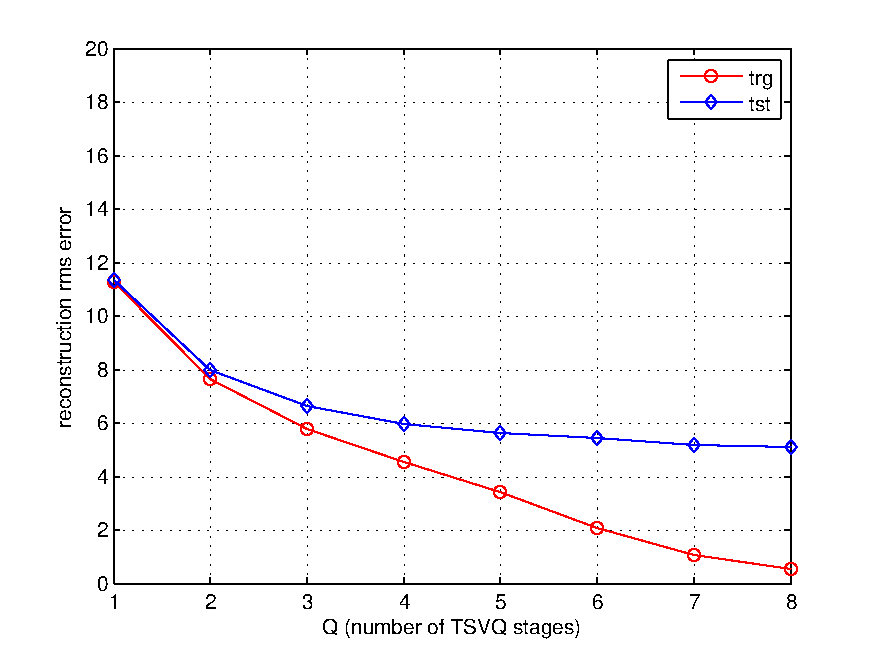
\includegraphics[width=0.45\textwidth]{thesis/TSVQ_Dudek.pdf}}
								\caption{TSVQ, 100 training examples in $\mathbb{R}^{1089}$ were used for each of these experiments. Results were averaged over 10 cross-validation runs. For each run, 20\% of the data, i.e., 20 examples were randomly picked for testing while the remaining 80 examples were used for training.}
								\label{fig:TSVQ_results}
								\end{figure}

Common appearance models include just the raw values of the pixel intensities~\cite{2000_CNF_TRK_Mallet, 1981_JNL_OpticalFlow_HornSchunck}, pixel intensity distributions~\cite{2002_JNL_MeanShiftFeatureSpaceAnalysis_Comaniciu, 1996_JNL_TRK_Zhu, 2002_JNL_TRK_Paragios, 2002_JNL_TRK_Elgammal}, templates\cite{1997_CNF_TRK_Fieguth}, active appearance models~\cite{1998_CNF_ActiveModels_Edwards, 1995_JNL_ActiveModels_Cootes}, pixel intensity centroids~\cite{1997_CNF_TRK_Heisele} and subspace based methods~\cite{1997_JNL_EigenTRK_Moghaddam, 1998_JNL_Eigentracking_Black}.  

In order to understand appearance modeling, we conduct the following 4 experiments using PCA, RVQ and TSVQ to measure rms errors for target reconstruction:

\begin{enumerate}
\item PCA: varying number of eigenvectors, $Q$.
\item RVQp: varying number of stages $P$ for RVQ while holding the number of code-vectors per stage constant at $M=4$.
\item RVQm: varying number of code-vectors per stage $M$ for RVQ while holding the number of stages constant at $P=8$.
\item TSVQ: varying number of stages, $P$.
\end{enumerate}

It is hoped that investigating reconstruction errors will aid in understanding the behavior of these various algorithms when used to model target appearance in tracking applications.

We use four datasets in $\mathbb{R}^{1089}$: (a) Uniform random variable, (b) Gaussian random variable, (c) Gauss-Markov random variable, and (d) images from the Dudek sequence. The reason for using $\mathbb{R}^{1089}$ is that our targets for all our tracking datasets are warped to a canonical size of 33-pixel height and 33-pixel width (33x33=1089). In all cases, we take 100 examples and split them up using an 80/20 rule, i.e. 80 training examples and 20 test examples. 10 cross-validation runs are used. In each cross-validation run, the training and test examples are picked randomly in the 80/20 ratio.

Results for PCA, RVQp, RVQm and TSVQ are shown in Figures~\ref{fig:PCA_results}, \ref{fig:RVQ_results_varyingP} \ref{fig:RVQ_results_varyingM} and \ref{fig:TSVQ_results} respectively.  We make the following observations from these figures:

\begin{enumerate}
\item \textbf{Training error}. Training error is always less than test error, as expected. Also, for each of the algorithms individually, we observe,
\begin{itemize}
\item \underline{PCA}: Monotonic decrease in rms reconstruction error with increasing $Q$. Training error becomes 0 when $Q=80$ since there are 80 training examples.
\item \underline{RVQp}: Monotonic decrease in rms reconstruction error with increasing $P$.
\item \underline{RVQm}: Monotonic decrease or approximately constant rms reconstruction error with increasing $M$.
\item \underline{TSVQ}: Monotonic decrease in rms reconstruction error with increasing $P$.
\end{itemize}
\item \textbf{Test error}.
\begin{itemize}
\item \underline{Statistically independent data}: For the uniform and Gaussian random variables, test error for PCA and RVQp stays almost constant with increasing $Q$ and $P$ respectively.  The reason is that PCA and RVQp use successive refinement when increasing $Q$ and $P$ respectively.  Test error is therefore not expected to get better since it is not possible to better explain random data with increasing $Q$ and $P$.

For RVQm and TSVQ, test error increases with increasing $M$ and $P$ respectively.  For TSVQ, increasing $P$ controls its VC (Vapnik-Chervonenkis) dimension~\cite{1999_BOOK_PRML_Vapnik} and therefore its generalization ability~\cite{2003_JNL_PRML_Karacali}.  It appears that increasing $M$ in RVQm has a similar effect.  The reason is that with $P=1$, increasing $M$ in RVQ is equivalent to increasing $P$ in TSVQ.  Increasing $P$ in RVQ adds additional refinement to the equivalent code-vectors but $M$ controls the overall general placement of RVQ code-vectors in the decision space $\mathbb{R}^D$.  Therefore, in RVQ, it is $M$ more than $P$ that controls generalization ability.  Therefore, when $M$ in RVQm or $P$ in TSVQ increase, their generalization ability decreases , leading to better explanation of training data, but with less ability to explain the test data well. For both RVQm and TSVQ, notice that when training error falls off sharply, test error increases sharply. Also, when training error drop is gradual, so is test error increase rate. This confirms over-training behavior. Also, RVQ increase or decrease rates are more gradual than TSVQ.  The reason is that for RVQm, the number of equivalent code-vectors increase as $2^8, 3^8, 4^8, \ldots, 10^8$.  Even for small values of $M$, the number of equivalent code-vectors is already quite large.  For TSVQ, the terminal code-vectors increase as $2^1, 2^2, 2^3, \ldots, 2^8$ and therefore there is a rapid increase in the number of code-vectors from a very small value to a very large value.

Finally, the rms reconstruction error is lower for uniform random data than for Gaussian random data.\footnote{It is may be tempting to explain this using an entropy argument.  The uniform distribution has the maximum entropy among all continuous distributions with finite support $[a,b]$ while the Gaussian distribution has maximum entropy among all distributions with infinite support~\cite{1982_JNL_MaxEntropy_Jaynes}.  However, due to the difference in support, it is difficult to compare entropies.} The reason is that the variance of the gaussian distribution is 1 while the variance of the uniform distribution with support $[0,1]$ is much lower at 1/12~\cite{1993_BOOK_RandomProcesses_Garcia}.
\item \underline{Statistically dependent data}: For the Gauss-Markov and Dudek cases, all 4 algorithms display decreasing test error with increasing $Q$ or $P$. The leveling off of the test error, or the "knee-point"~\cite{2009_BOOK_PRML_Escolano}, is visible in all cases.
\end{itemize}
\end{enumerate}
In these experiments, we see that training error of PCA is in general better than RVQ. This is expected since PCA can achieve perfect reconstruction when $Q$ comes close to the number of training examples $N$, $N<<D$.  Test errors however are comparable.  RVQ has 2 knobs, $P$ and $M$. In varying $P$, it acts like PCA in providing successive approximation. In varying $M$, it acts like TSVQ in changing its VC dimension, and therefore its generalization ability.  Given this flexibility, it is expected that RVQ will perform well in our tracking framework.

%=======================		
\section{Model 2: Observation model}
%=======================
								\begin{figure}[t]
								\centering
								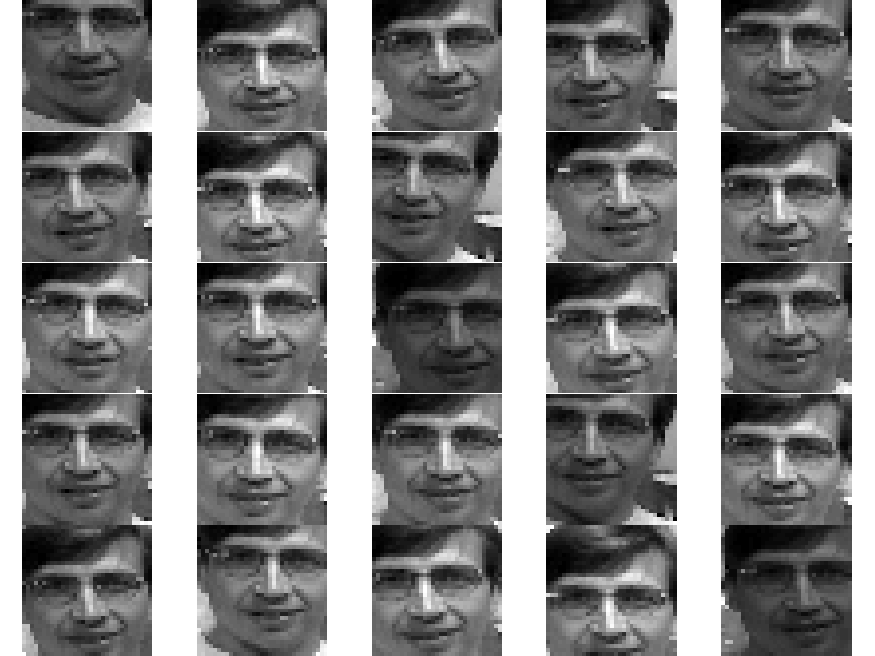
\includegraphics[width=0.65\textwidth]{thesis/affineCandidates.pdf}
								\caption{Different observations extracted from the frame at time $t$ that will be evaluated to find the snippet that is best explained by the appearance model.  The brightness changes in the various snippets is due to scaling.}
								\label{Fig:affine_candidates}
								\end{figure}

An observation model $p(z_t|x_t)$ relates the state $x_t$ at time $t$ to the observation $z_t$ at time $t$.  Unfortunately, it is not possible to estimate the observation model from the data and so reasonable assumptions must be made.  The observations are assumed to be independent of each other as well as of the dynamical process \cite{1998_JNL_Condensation_IsardBlake}. 

%In this work, for PCA, the observation model assumes that the candidate window chips (snippets) in the image that can contain the target were generated from a subspace of the target $\mathbf{U}$ centered at $\mathbf{\mu}$.  For RVQ and TSVQ, the observation model assumes that the candidate snippets were generated from the RVQ and TSVQ codebooks respectively.  

In the first step, the observation model generates observations that will serve as candidates for the target, as shown in Figure~\ref{Fig:affine_candidates}.  

For PCA, it is assumed that an image $\mathbf{x}$ in $\mathbb{R}^D$ is probabilistically generated from a subspace $\mathbf{U}$ spanned by earlier observed images.  The covariance matrix $\Sigma$ of the input training images can be written as $\Sigma = \mathbf{U}\mathbf{\Lambda} \mathbf{V}^T$.  Here $\mathbf{\Lambda}$ is the matrix of eigenvalues.  The distribution is assumed to be Gaussian centered at $\boldsymbol{\mu}$.  The probability of an image being generated under this distribution is inversely proportional to its distance from $\boldsymbol{\mu}$.  This distance can be decomposed into two parts:

\begin{enumerate}
\item DFFS (distance-from-feature-space):  In a partial KL expansion using $Q$ eigenvectors, the space spanned by these $Q$ eigenvectors is given by $\mathbf{F}$\footnote{We use $\mathbf{U}$ interchangeably with $\mathbf{F}$ here.  Whereas the notation $\mathbf{U}$ is more widely used to represent a PCA eigenspace, we use $\mathbf{F}$ to remain compatible with Figure~\ref{fig:1997_JNL_DIFSDFFS_Moghaddam} taken from ~\cite{1997_JNL_EigenTRK_Moghaddam}.} and the signal residual $\epsilon^2$ is given by

\begin{equation}
\epsilon^2 = \Vert \tilde{\mathbf{x}} \Vert^2 - \sum\limits_{i=1}^Q \mathbf{u}_i^2 = \sum\limits_{i=Q+1}^D \mathbf{u}_i^2
\end{equation}

where $\tilde{\mathbf{x}}$ is the mean removed input image and $\mathbf{u}_i$ are the eigenvectors of the covariance matrix estimate, $\boldsymbol\Sigma=\tilde{\mathbf{x}}\tilde{\mathbf{x}}^T$  .  This signal residual is referred to as DFFS.
\item DIFS (distance-in-feature-space):  This is the component of $\mathbf{x}$ which lies in the feature space $\mathbf{F}$.  
\end{enumerate}

DIFS and DFFS are illustrated graphically in Figure~\ref{fig:1997_JNL_DIFSDFFS_Moghaddam}.  In a gaussian distribution, the probability of a data point $\mathbf{x}$ in $\mathbb{R}^D$ depends on the Mahalanobis distance $d$.  The output of PCA, zero-centered $\mathbf{\tilde{y}}$ is decorrelated with variances along each dimension equal to the eigenvalues $\lambda_i$ of the covariance matrix $\boldsymbol\Sigma$,


\begin{equation}
\begin{array}{lllllll}
d &= (\mathbf{x}-\boldsymbol\mu)^T\boldsymbol\Sigma^{-1}(\mathbf{x}-\boldsymbol\mu)\\
&=\mathbf{\tilde{x}}^T\boldsymbol\Sigma^{-1}\mathbf{\tilde{x}}\\
&=\mathbf{\tilde{x}}^T(\mathbf{U}\boldsymbol\Lambda\mathbf{U}^T)^{-1}\mathbf{\tilde{x}}\\
&=\mathbf{\tilde{x}}^T(\mathbf{U}\boldsymbol\Lambda^{-1}\mathbf{U}^{-1})\mathbf{\tilde{x}}\\
&=(\mathbf{U}^T\mathbf{\tilde{x}})^T\boldsymbol\Lambda^{-1}(\mathbf{U}^T\mathbf{\tilde{x}})	\\
&=\mathbf{\tilde{y}}^T\boldsymbol\Lambda^{-1}\mathbf{\tilde{y}}\\
&=\sum\limits_{d=1}^D \frac{\tilde{y}_i}{\lambda_i}\\
&=\sum\limits_{d=1}^Q \frac{\tilde{y}_i^2}{\lambda_i} + {\color{red}\sum\limits_{d=Q+1}^D} \frac{{\color{red}\tilde{y}_i^2}}{\lambda_i}, \ \ \  & \bigg(\textrm{DFFS = recon. error}={\color{red}\sum\limits_{i=1}^D e_i^2} = \sum\limits_{i=1}^D \tilde{x}_i^2 - \sum\limits_{i=1}^Q \tilde{y}_i^2= {\color{red}\sum\limits_{d=Q+1}^D} {\color{red}\tilde{y}_i^2}\bigg)\\
&=\sum\limits_{d=1}^Q \frac{\tilde{y}_i^2}{\lambda_i} + \frac{1}{\rho} {\color{red}\sum\limits_{i=1}^D e_i^2} \ \ \ & \bigg(\rho^* = \frac{1}{D-q}\sum\limits_{i=q+1}^D \lambda_i\bigg)\\
\end{array}
\label{Eqn:MoghaddamLikelihood}
\end{equation}

This formulation, first presented in~\cite{1997_JNL_EigenTRK_Moghaddam} shows that the first term in the sum is the DIFS term in Figure~\ref{fig:1997_JNL_DIFSDFFS_Moghaddam} while the second term corresponds to DFFS.  With this formulation, PCA can be used in a probabilistic framework since the error of a test vector $\mathbf{x}$ now also depends on its distance from the mean of the data.  However, as mentioned in~\cite{2008_JNL_subspaceTRK_Ross}, it is difficult to weight these two terms.  In this work, we therefore only use DIFS so that our approach does not rely on finding different weights for different datasets.


%This leads the likelihood function to be a function of two distributions,
%
%\begin{equation}
%p(\mathbf{I}|\mathbf{X}) =  \mathcal{N}()
%\end{equation}
%
%\begin{equation}
%p(I_t|X_t) = \mathcal{N}
%\end{equation}


%The candidate that gives least mean squared error is chosen as the most likely to find the terminal code-vector in the TSVQ tree that minimizes mean-squared error.  

As mentioned earlier, VQ, like PCA, does not define a proper density in the observation space~\cite{1999_JNL_Gaussian_roweis}.  However, it is common to assign a probability measure to a new data point in proportion to the distance of the closest centroid~\cite{1999_JNL_Gaussian_roweis},

\begin{equation}
p(\mathbf{x}_i|\boldsymbol\mu_k) = \frac{e^{-\big(\dr\big)}} {\sum\limits_{i=1}^N e^{-\big(\dr\big)}}
\end{equation}

Here, $\boldsymbol\mu_k$ is the closest code-vector to test data-point to $\mathbf{x}_i$,  $P_{\textrm{max}}$ is the number of stages in the codebook, $P_i$ is the number of stages required to decode $\mathbf{x}_i$, and $\lambda$ is a regularization parameter.  We use 4 different RVQ methods to compute which $\boldsymbol \mu_k$ input data-point $\mathbf{x}_i$ maps to,

\begin{enumerate}
\item \underline{maxP}: In this method, RVQ decoding is carried out so that maximum stages $P$ are used.
\item \underline{RofE}: In this method, realm of experience coding is used.  In other words, a test vector is decoded such that the decode path traversed belongs to the set of training decode paths.
\item \underline{nulE}: In this method, null encoding is used.  Reconstruction rms error is checked at every stage.  If at any stage, rms error is not reduced, that stage is skipped.
\item \underline{monR}: In this method, monotonic rms error is a condition.  If this condition is not met, decoding stops.
\end{enumerate}

In our tracking framework, we use all 4 methods above and compare their performance. 

%=======================		
\section{Model 3: Representation model}
\label{Sec:Representation_model}
%=======================
%\begin{itemize}
%\item \underline{Temporary occlusions}.  The occlusions are temporary, on the order of about 10 frames.
%\end{itemize}
%\begin{itemize}
%\item \underline{Perspective changes handled effectively with affine deformation}.  An affine transform in a tracking scenario can deal effectively with a large variety of target deformations, including some perspective effects.  We therefore choose the affine transform in favor of the less restrictive projective transform which can handle severe perspective effects.  A comparison of some 2D geometric transformations is given in Table~\ref{table:2Dtransformations}.
%\end{itemize}		
In this section, we discuss the representation model.  See also Figure~\ref{fig:TRK_objectRepresentations} in the introductory chapter that shows different target representations.  In many situations, it is necessary to track a visual target that is undergoing deformations.  Several targets of interest fall in this category, particularly non-rigid targets such as humans.  Even rigid objects can undergo deformation in a matter of seconds as shown in Figure~\ref{Fig:PETS2001_deformation}.  

								\begin{table}[t]
								\centering
								\begin{tabular}{| l | c | c | p{2.5in} |}
								\hline
								Transformation & DoF & Matrix & Distortion\\ \hline 
								& & & \\ Projective & 8 & $\ProjMatrix$ & any arbitrary quadrilateral as long as no three points are collinear\\  & & & \\ \hline
								& & & \\ Affine & 6 & $\AffMatrix$ & rotation and non-isotropic scaling\\  & & & \\ \hline
								& & & \\ Similarity & 5 & $\SimMatrix$ & scaling and rigid motion\\  & & & \\ \hline
								& & & \\ Euclidean & 4 & $\EucMatrix$ & rigid motion (rotation, translation) \\  & & & \\ \hline
								\end{tabular}\
								\caption{2D transformations}
								\label{table:2Dtransformations}
								\end{table}

								\begin{figure}[t]
								\centering
								\subfigure[Frame 770.]{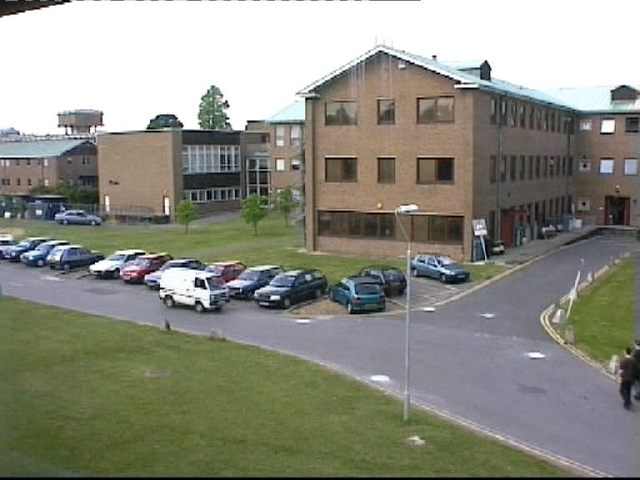
\includegraphics[width=0.45\textwidth]{thesis/PETS2001_00770.jpg}}
								\subfigure[Frame 1770.]{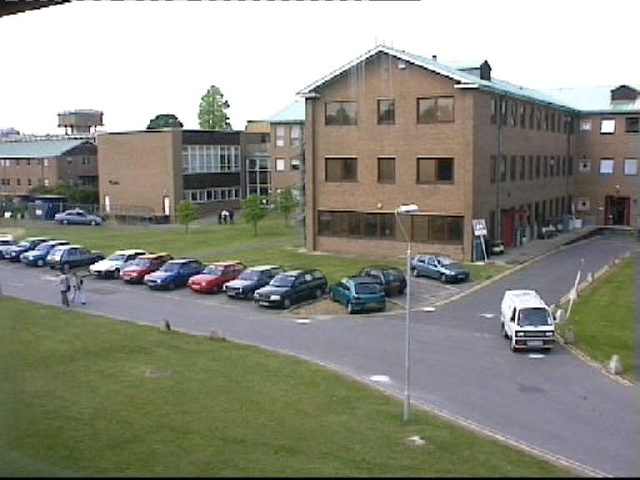
\includegraphics[width=0.45\textwidth]{thesis/PETS2001_01770.jpg}}
								\caption{Over time, even rigid objects can undergo deformations such as the car in these images from the PETS2001 dataset.}
								\label{Fig:PETS2001_deformation}
								\end{figure}

								\begin{figure}[t]
								\centering
								\subfigure[Affine parameters $(\theta, \lambda_1, \lambda_2, \phi, x, y)$ corresponding to the bounding box and a few feature points are manually selected.]{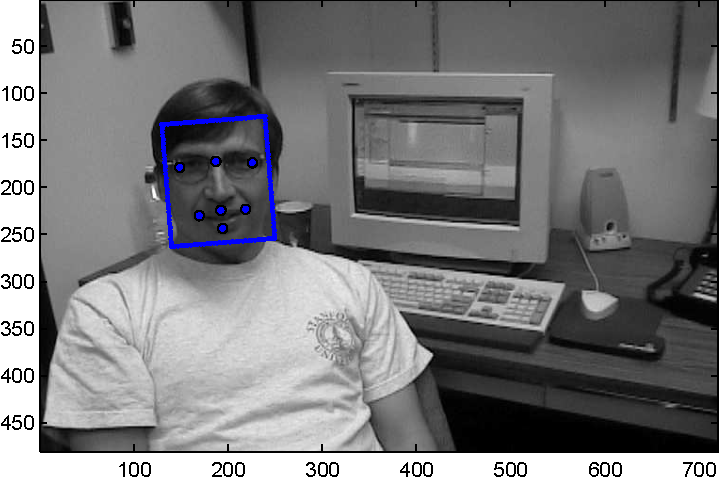
\includegraphics[width=0.65\textwidth]{thesis/dataset_Dudek_with_feature_points_00001.pdf}}\\
								\subfigure[Reference position of feature points.]{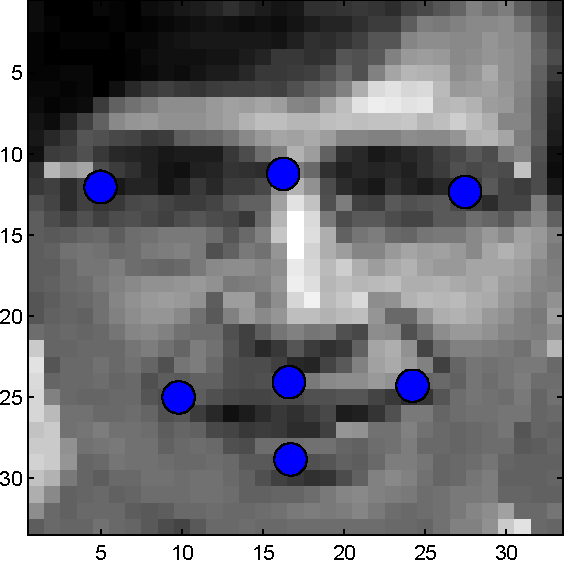
\includegraphics[width=0.25\textwidth]{thesis/dataset_Dudek_desired_00001.pdf}}
								\caption{Manual target initialization in the first frame.  The manually selected target and manually selected feature points (top image) are warped to an upright reference position using $(\theta, \lambda_1, \lambda_2, \phi, x, y)$.  The position of these feature points (lower figure) is kept as reference throughout the tracking process.}
								\label{Fig:affine_frame_1}
								\end{figure}

								\begin{figure}[t]
								\centering
								\fbox{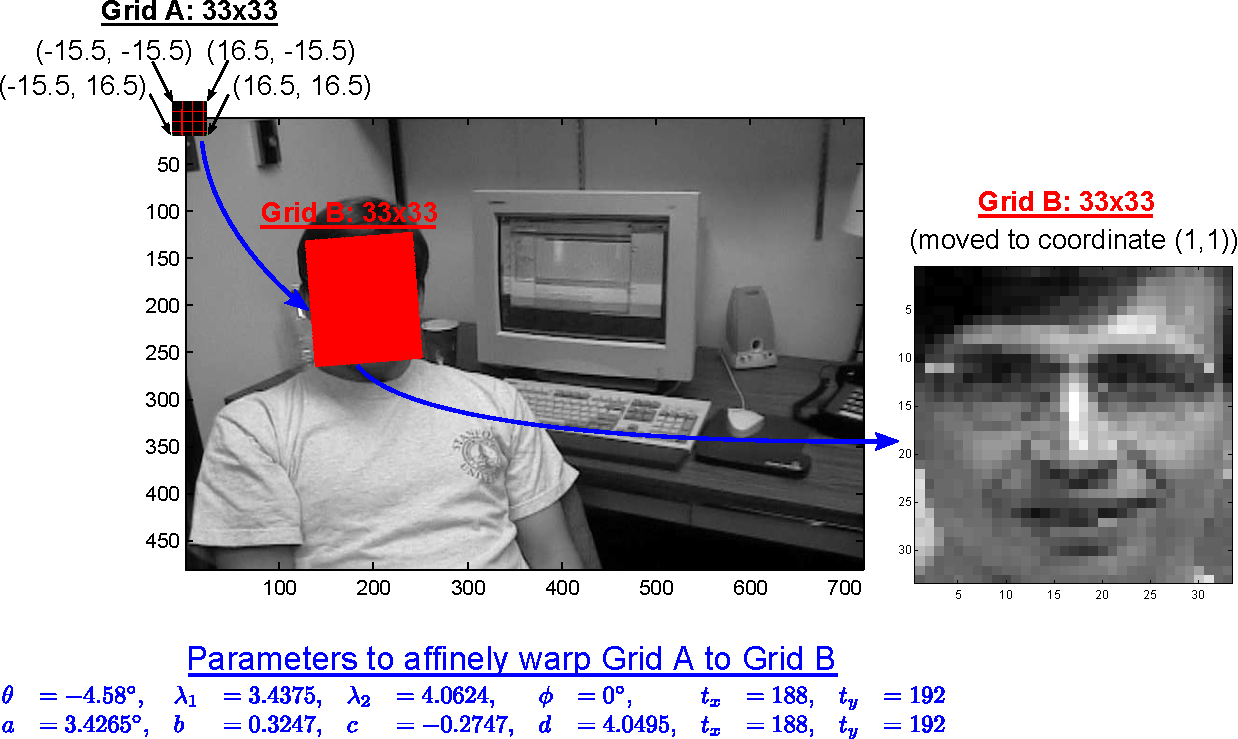
\includegraphics[width=0.85\textwidth]{thesis/dataset_Dudek_00001_forwardAffine.pdf}}
								\caption{Run-time processing.  A zero-centered grid is warped using a given set of affine parameters to cover the object of interest.  Pixel intensities at the warped grid points are computed using bilinear interpolation.}
								\label{Fig:affine_runtime}
								\end{figure}

In such cases, using a rigid rectangular bounding box to represent the target will inevitably lead to inclusion of background pixels in the matching process.  This can easily lead to tracker drift, particularly if the tracker is also trying to learn the appearance model of the target.

We now show how to use affine warping of the rectangular bounding box so that it more closely captures the outline of the target of interest.  This minimizes inclusion of background pixels in the matching process and leads to more robust tracking.

Table \ref{table:2Dtransformations} shows different kinds of 2D linear transformations.  Every transformation generalizes the transformation below it in the table.  In this report, we are interested in the 2D affine transform since it is flexible enough to account for most distortions in real images.

The affine transform\footnote{The notation adopted by some books for the affine transform is,

\begin{equation}
\begin{array}{llllllll}
X &= ax + by + e\\
Y &= cx + dy + f
\end{array}
\label{Eq:AffineDecomposition}
\end{equation}

where the input coordinate (x,y) has been transformed through 6 affine parameters, $a, b, c, d, e, f$ to the output coordinate $(X,Y)$.  Instead of $e$ and $f$, we will be using $x$ and $y$ respectively.}
 is given by,

\begin{equation}
\begin{array}{cllll}
\left[\begin{array}{l}\acute{x}\\\acute{y}\\1\end{array}\right]   &=& \AffMatrix \left[\begin{array}{l}x\\y\\1\end{array}\right]\\
\mathbf{\acute{x}} &=& \left[\begin{array}{cccc}\mathbf{A} & \mathbf{t}\\\mathbf{0}^T & 1\end{array}\right] \mathbf{x}\\
&=& \mathbf{A}\mathbf{x} + \mathbf{t}\\
&=& \mathbf{H}_A \mathbf{x}\\
\end{array}
\label{Eqn:top_level}
\end{equation}

$x$ and $y$ are translations in the $x$ and $y$ directions respectively and $\mathbf{H}_A$ is the affine transformation matrix.  The matrix $\mathbf{A}$ above can always be decomposed using the SVD decomposition as the product of orthonormal matrix $\mathbf{U}$ containing the eigenvectors of $\mathbf{A}\mathbf{A}^T$, orthonormal matrix $\mathbf{V}$ containing the eigenvectors  $\mathbf{A}^T\mathbf{A}$ and a diagonal matrix $\mathbf{S}$ containing the eigenvalues of $\mathbf{A}$~\cite{2004_BOOK_CG_Hartley}:

\begin{equation}
\begin{array}{llllllll}
\mathbf{A} &= \left[\begin{array}{lll}a & b \\ c & d\\ \end{array}\right] \\
&=\mathbf{U}{\color{darkgreen}\mathbf{S}}{\color{red}\mathbf{V}^t} \\
&={\color{blue}(\mathbf{U}\mathbf{V}^t)}{\color{red}\mathbf{V}}{\color{darkgreen}\mathbf{S}}{\color{red}\mathbf{V}^t}\\
&={\color{blue}\mathbf{R}(\theta)}{\color{red}\mathbf{R}(-\phi)}{\color{darkgreen}\mathbf{S}}{\color{red}\mathbf{R} (\phi)}\\
&={\color{blue}\RotMatrixTheta}{\color{red}\RotMatrixminusPhi}{\color{darkgreen}\EigenvalueMatrix}{\color{red}\RotMatrixPhi}\\\\
\end{array}
\label{Eq:AffineDecomposition}
\end{equation}

${\color{blue}\mathbf{U}\mathbf{V}^t}$ is an orthogonal matrix since $({\color{blue}\mathbf{U}\mathbf{V}^t})^t =({\color{blue}\mathbf{U}\mathbf{V}^t})^{-1}$.  Therefore, without loss of generality, it can be written as a rotation matrix.  Of the possible 6 DOFs (degrees of freedom) of the affine transformation, the 4 DOFs in $\mathbf{A}$, i.e., ($a, b, c$, $d$) have been replaced with $(\theta, \lambda_1, \lambda_2, \phi)$.

The affine matrix $\mathbf{A}$ can therefore be viewed as a succession of the following 4 steps: (a) Rotation by angle $\phi$, (b) scaling of $\lambda_1$ and $\lambda_2$ in the rotated $x$ and $y$ directions, (c) rotation by angle -$\phi$ which brings the scaled object back to its original orientation, and (d) rotation by angle $\theta$.  We now discuss how to convert between affine parameter representations.

\begin{enumerate} 
\item \underline{Converting $(a, b, c, d)$ to $(\theta, \lambda_1, \lambda_2, \phi)$}.  In several cases, the affine parameters are given in the form of $(a, b, c, d)$.  However, it is difficult to get a physical intuition when the parameterization is done in this form.  In such cases, converting to $(\theta, \lambda_1, \lambda_2, \phi)$ helps in getting an insight into how the object of interest is being deformed.  Also, for the particle filter, it is more intuitive to specify expected variances for $(\theta, \lambda_1, \lambda_2, \phi)$ than for $(a, b, c, d)$.  The first step here is to compute the SVD decomposition $\mathbf{A}=\mathbf{U}{\color{darkgreen}\mathbf{S}}{\color{red}\mathbf{V}^t}$.  The parameters $(\theta, \lambda_1, \lambda_2, \phi)$ are computed as follows,

\begin{equation}
\boxed{
\begin{array}{llll}
\phi &=& \tan^{-1}\frac{v_{1,2}}{v_{1,1}}\\
\lambda_1 &=&  s_{1,1}\\
\lambda_2 &=& s_{2,2}\\
\theta &=& \tan^{-1}\frac{u_{2,1}v_{1,1} + u_{2,2}v_{1,2}}{u_{1,1}v_{1,1} + u_{1,2}v_{1,2}}
\end{array}}
\end{equation}

\item \underline{Converting  $(\theta, \lambda_1, \lambda_2, \phi)$ to $(a, b, c, d)$}.  In visual tracking, the initial target planar bounding region is more intuitively expressed in terms of $(\theta, \lambda_1, \lambda_2, \phi)$ than in terms of $(a, b, c, d)$.  However, the actual affine warp is more easily carried out using matrix multiplication for which we need $(a, b, c, d)$.  This can be done by multiplying out all the terms in Equation~\ref{Eq:AffineDecomposition} to get

\begin{equation}
\boxed{
\begin{array}{llll}
a &= (\lambda_2) p + (\lambda_1) q\\
b &= (\lambda_2) s  - (\lambda_1) r \\
c &= (\lambda_2) r  - (\lambda_1) s \\
d &= (\lambda_2)q + (\lambda_1) p
\end{array}}
\label{Eqn:tllpxy_to_abcdxy}
\end{equation}

where temporary variables $p, q, r, s$ are computed from angles $\theta$ and $\phi$ using~\cite{2008_JNL_subspaceTRK_Ross},

\begin{equation}
\begin{array}{llll}
\mathrm{ccc} = \cos(\theta) \cos^2(\phi), \mathrm{ccs} = \cos(\theta) \cos(\phi) \sin(\phi), \mathrm{css} = \cos(\theta) \sin^2(\phi)\\
\mathrm{scc} = \sin(\theta) \cos^2(\phi), \mathrm{scs} = \sin(\theta) \cos(\phi) \sin(\phi), \mathrm{sss} = \sin(\theta) \sin^2(\phi)\\
p   =  \mathrm{css} - \mathrm{scs}, q   =  \mathrm{ccc} + \mathrm{scs}, r  = \mathrm{ccs} + \mathrm{sss}, s =  \mathrm{ccs} - \mathrm{scc}\\
\end{array}
\end{equation}
\end{enumerate}

During tracking, in the first frame, manually selected affine parameters and feature points are warped to an upright reference position as shown in Figure~\ref{Fig:affine_frame_1}.  During run-time, in every frame, the motion model (discussed next) generates several affine candidate parameter sets.  Each of these sets is used to warp a zero-centered grid onto or around the object of interest.  Bilinear interpolation is then used to compute pixel intensity values at the warped grid points as shown in Figure~\ref{Fig:affine_runtime}.  For the example affine parameter set given in this figure, we see that the affinely warped region accurately samples the object of interest and minimizes inclusion of background pixels.  Tracking error for a particular affine parameter set in a frame can be computed by warping the reference feature points from the first frame using this affine parameter set and computing rms error with ground truth feature points for that frame.  We now discuss the motion model.

%=======================		
\section{Model 4: Motion model}
%=======================		
The motion model is a mathematical representation of the real or expected motion of the target of interest.  Since tracking is in general an ill-posed problem, it is common to make assumptions about the motion to simplify motion modeling.  Common assumptions such as stationary camera, coherent motion etc. are discussed in Chapter~\ref{chap_TRK}.

In this work, we make two assumptions about the target motion:

\begin{itemize}
\item \underline{Coherent motion}.  We assume that each part of the target moves together.  The target can deform and warp but it does not break up into individual parts.
\item \underline{Can be modeled with a gaussian distribution with fixed variance}.  We assume that the motion is brownian and can be modeled with a gaussian distrubution with a fixed variance.  
\end{itemize}

An advantage of not having an explicit motion model is that arbitrary camera and target motion are allowed.  A disadvantage of this approach in the context of the particle filter is that particles need to be evaluated all around the current target position, rather than around a predicted target position in a certain direction.  We are therefore unable to take advantage of the reduced spatial search-space that comes with a deterministic motion model.  

At time $t$, the goal of the tracking process is to estimate the state vector $\mathbf{X}_t = (\theta, \lambda_1, \lambda_2, \phi, x, y)$.  To keep our model as general as possible, all 6 components of the state vector are modeled as Gaussian random variables but with known variance which is specified in the first frame.  However, in order to simplify sampling from the joint density, it is possible to use certain relaxation criteria such as Markovian dependence, or independence.  We choose the latter to avoid MCMC sampling~\cite{2009_BOOK_Bayes_Hoff} and note that this method works well in practice.  The target motion is therefore represented not in analytic form but as a 6x6 diagonal covariance matrix $\Sigma_X$ centered at $\mathbf{X}_{t-1}$ in the previous frame.  The elements on the diagonal represent variances of the affine parameters, $\sigma_\theta^2, \sigma_{\lambda_1}^2, \sigma_{\lambda_2}^2, \sigma_\phi^2, \sigma_x^2, \sigma_y^2$.  For instance, for the $x$ and $y$ coordinates of the target at time $t$, the probability of the target position is given by,

\begin{align}
p(x_t|x_{t-1}) &= \mathcal{N}(x_{t-1}, \sigma_x^2) \\
p(y_t|y_{t-1}) &= \mathcal{N}(y_{t-1}, \sigma_y^2)
\end{align}

At every time step, predicted values are sampled from all 6 distributions.  Each predicted set is used to warp a zero-centered grid onto or around the target of interest as explained in the previous section.  Next, we discuss the inference model which is used to select the best set of affine candidates generated by the motion model.

%=======================		
\section{Model 5: Inference model}
%=======================	
								\begin{figure}[t]
								\centering
								\subfigure[Reference (uniform) density and test PDF.]{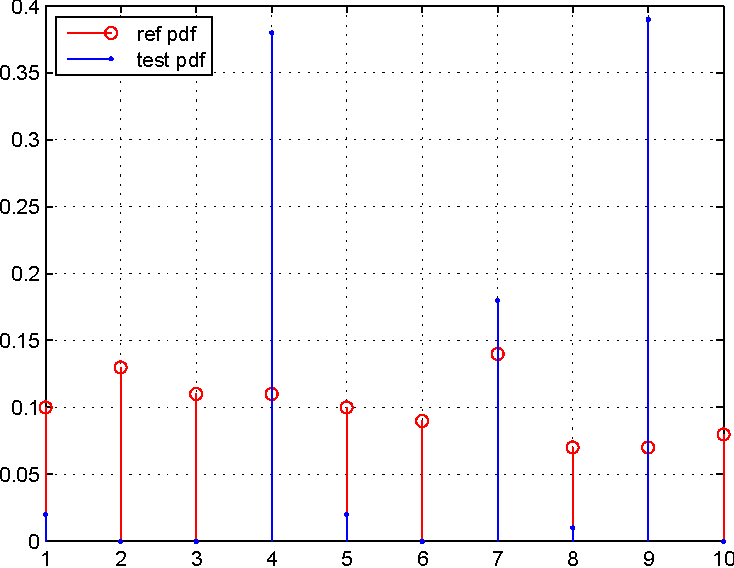
\includegraphics[width=0.4\textwidth]{thesis/particle_filter_pdfs.pdf}}
								\subfigure[Comparing CDFs.]{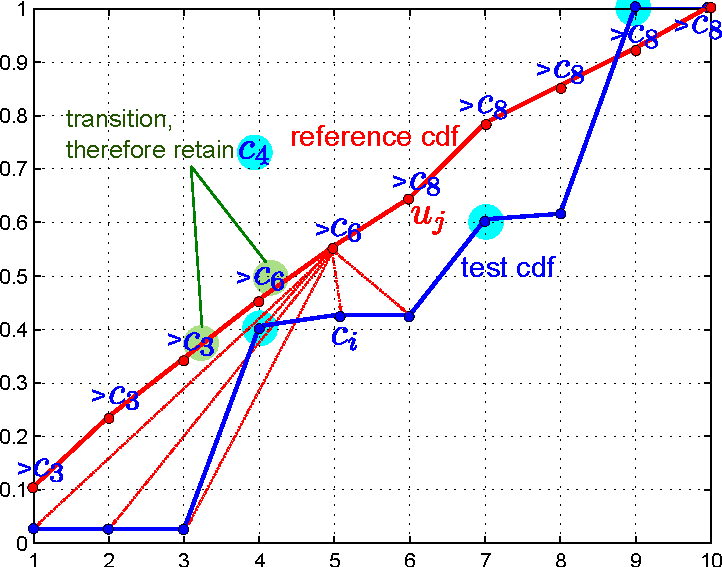
\includegraphics[width=0.4\textwidth]{thesis/particle_filter_resampling.pdf}}
								\subfigure[Particles 4, 7 and 9 are picked repeatedly since they have higher weight.]{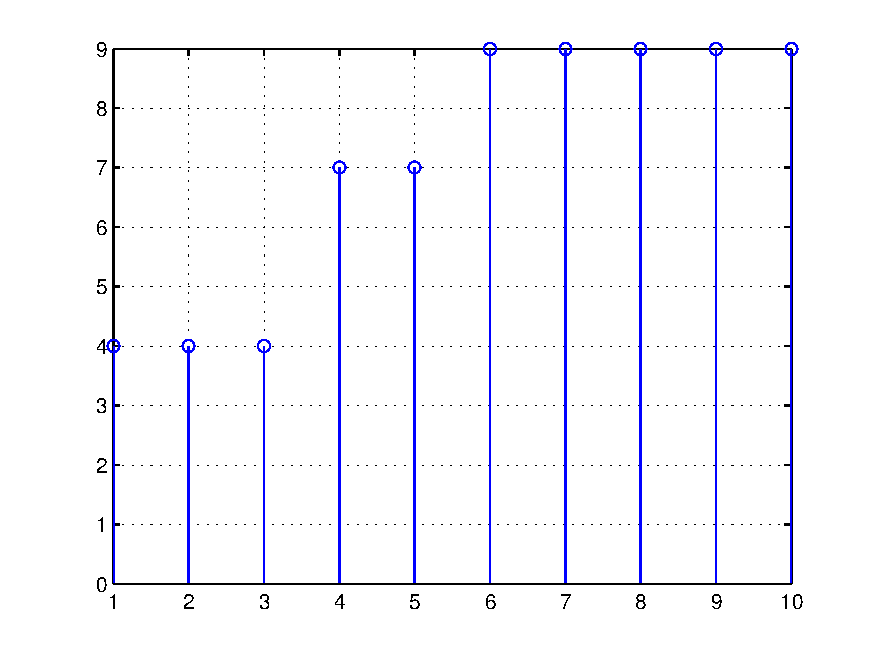
\includegraphics[width=0.45\textwidth]{thesis/particle_filter_particles.pdf}}
								\caption{Particle filter, resampling.}
								\label{fig:particle_filter_resampling}
								\end{figure}

The inference model makes the final decision of which candidate snippet to pick as the target.  Our inference model makes no assumption of linearity or Gaussianity.  What this means is that we do not assume that the motion or observation models are linear, nor do we assume that the likelihood of finding a target at a particular location has a Gaussian distribution.  Morever, we would like to keep a history of possible target candidate states, 600 in this case, so that soft decisions can be made about the target state at each frame.  In other words, at every frame, even though we make a decision as to which particular snippet best represents the target, we acknowledge that this decision could be erroneous and therefore we propagate other candidates through time.  This allows us to revisit candidate snippets that were not picked in previous frames as the target estimate but that could still have a high probability of being the correct snippet.  Also, we do not want our hypotheses to grow with time.  Keeping all this in mind, we base our inference model on the sequential Monte Carlo (SMC) filter, i.e., the particle filter~\cite{2002_JNL_PF_Arulampalam}.  

As mentioned earlier, the weights of the target candidate snippets are computed in the observation model.  An example scenario using only 10 candidate snippets, i.e., particles, at time $t$ is given in Figure~\ref{fig:particle_filter_resampling}.  The test pdf in this figure is generated by normalizing the weights of the target candidate snippets.  In the first step, the inference model picks the 9th snippet as the target estimate since it has highest weight.  In the second step, the inference model resamples the test pdf to remove snippets that have low weight and to repeat snippets that have high weight.  To do this, a reference uniform density is generated.  The CDFs of these 2 densites are then compared.  Only those snippets are kept and repeated that have high weight as shown in the figure.  The new resampled density is then passed to the motion model to generate candidate snippets in the next frame.

Having explained all 5 models that constitute our tracking framework, we now apply our tracker to several image datasets and present our results.
%For a set of $N$ input points, a set $S$ of $N$ points is created such that each of these points $s_i$ corresponds to the $i$th index of the input CDF Those input points $x_i$ are picked for which the corresponding CDF points, $c_i$ induce a transition in the $i-th$ 
%\cite{1992_JNL_MCMC_Carlin}

%=========================
\section{Results}
%=========================


\begin{table}[t]
\footnotesize
\begin{tabular}{p{0.6in}|p{0.6in}p{0.6in}p{0.4in}p{0.4in}cccccc}
Dataset 		&Scenario	     &\parbox[c]{0.4in}{\center Time of \\day} 	&\parbox[c]{0.26in}{\center Target of \\interest}  &\parbox{0.3in}{\center Rigid \\target} 	&\parbox{0.4in}{\center Lighting change 1-5 \\(5 most severe)}  	&\parbox{0.5in}{\center Structured \\noise} 	&\parbox{0.4in}{\center Camera \\motion} 	&\parbox{0.3in}{\center Pose \\change} 	&\parbox{0.45in}{\center Expression \\change} 	&\parbox{0.3in}{\center Temporary \\occlusion} 	\\\hline
Dudek 			&Indoors 	     &N/A 			&human 					&no 	&1 	&yes 	&yes 	&yes 	&yes 	&yes 		\\\hline
davidin300 	&Indoors		&N/A			&human					&no	&2	&yes	&yes	&yes	&yes	&no		\\\hline
sylv				&Indoors		&N/A			&toy						&yes	&4	&no	&yes	&yes	&N/A	&no		\\\hline
trellis70	 		&Outdoors 		&day, dark		&human					&no	&5	&no	&yes	&yes	&yes	&no		\\\hline
fish				&Indoors		&N/A			&object					&yes	&4	&no	&yes	&no	&N/A	&no		\\\hline
car4			&Outdoors 		&day, sunny	&vehicle					&yes	&3	&no	&yes	&yes	&N/A	&no		\\\hline
car11			&Outdoors		&night			&vehicle					&yes	&4	&no	&yes	&yes	&N/A	&no		\\\hline
\end{tabular}
\caption{Datasets used for RVQ tracking.}
\label{Tab:datasets_used}
\end{table}

Here, we present tracking error results for our 6 different trackers, PCA-based, TSVQ-based and 4 RVQ-based trackers, maxP, RofE, nulE, and monR.


								\begin{figure}[t]
								\centering
								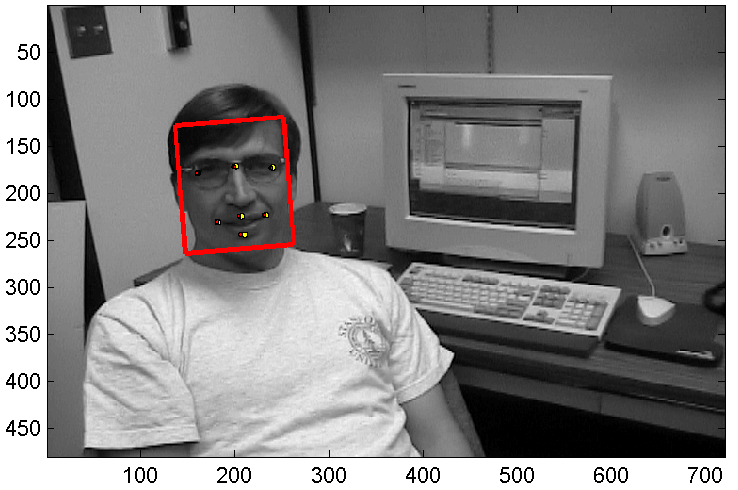
\includegraphics[width=0.7\textwidth]{thesis/results_pca__trk_dudek_0007.png}
								\caption{Computing tracking error.  The larger yellow circles indicate ground truth feature points.  The smaller red circles indicate estimated feature points.  Tracking error is computed using the rms error between the ground truth feature points and the estimated feature points.  In this particular frame, the tracking error is 2.57.}
								\label{fig:results_pca__trk_dudek_0007}
								\end{figure}

We have previously described our 5-component tracker comprising appearance, observation, representation, motion and inference models.  All 6 trackers share exactly the same representation, motion and inference models.  However, each has its own appearance and observation models.

All trackers were run on 6 publicly available datasets, Dudek, davidin300, sylv, fish, car4 and car11.  See Figure~\ref{fig:trk_sequences} in Appendix~\ref{App:dataset_snapshots} for snapshots of images in each dataset at 100 image intervals and Table~\ref{Tab:datasets_used} for the various challenges in these datasets.  These datasets can be downloaded from~\cite{2008_JNL_subspaceTRK_Ross}.  Tracking error was measured on each of these datasets using the error between ground truth feature points and estimated feature points as shown in Figure~\ref{fig:results_pca__trk_dudek_0007} for the Dudek sequence.

								\begin{figure}[t]
								\centering
								\begin{tabular}{|l|c|c|c|c|c|c|}
\hline
&\textbf{PCA}&\textbf{TSVQ}&\textbf{maxP}&\textbf{RofE}&\textbf{nulE}&\textbf{monR}\\\hline
\textbf{Dudek}&7.44&8.62&7.78&7.11&7.97&8.73\\\hline
\textbf{davidin300}&4.60&5.93&4.47&5.74&4.63&4.15\\\hline
\textbf{sylv}&4.34&4.61&4.00&4.12&4.74&4.31\\\hline
\textbf{fish}&2.17&4.59&2.78&2.73&2.48&2.89\\\hline
\textbf{car4}&4.60&5.11&4.67&4.93&5.28&4.71\\\hline
\textbf{car11}&2.13&2.21&2.17&2.33&2.52&2.47\\\hline
\textbf{ \% best}&50.00&0.00&16.67&16.67&0.00&16.67\\\hline
\end{tabular}

								\subfigure[Best tracking error for each algorithm.]{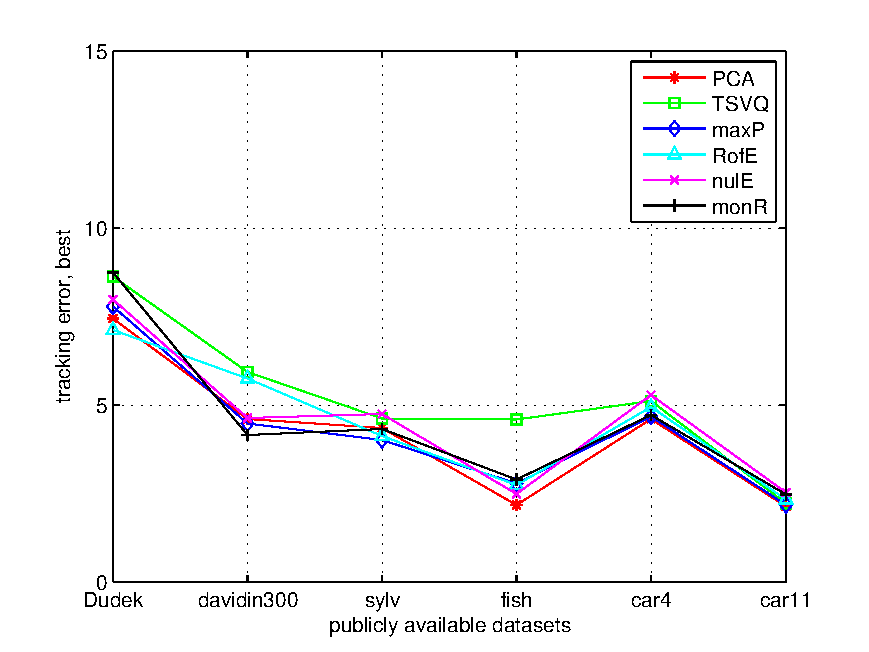
\includegraphics[width=0.47\textwidth]{thesis/results_final_1a_best.pdf}\label{fig:results_final_1a_best}}
								\subfigure[\%age of datasets over which best tracking error is achieved over all parameters.]{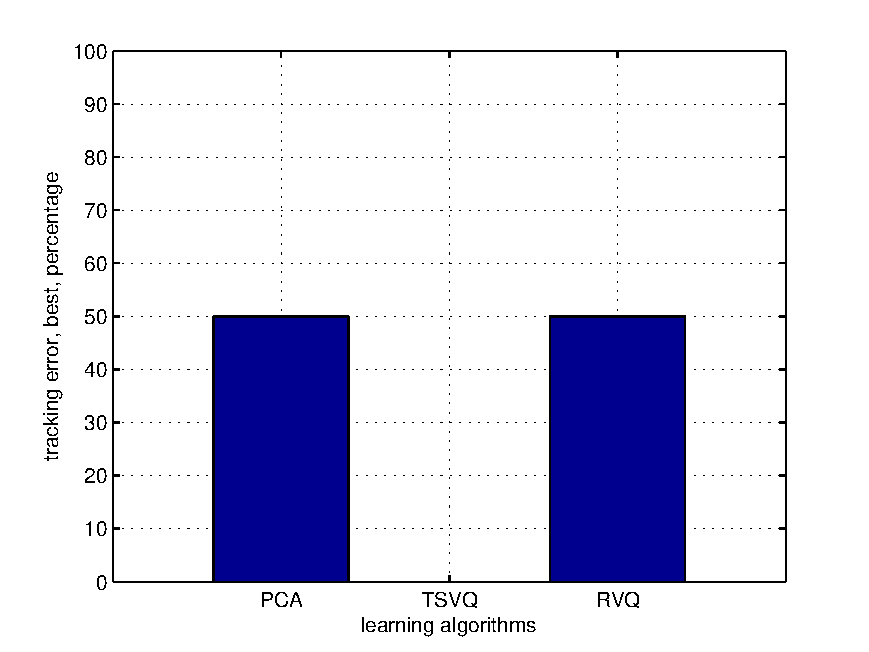
\includegraphics[width=0.47\textwidth]{thesis/results_final_1b_best_percent.pdf}\label{fig:results_final_1b_best_percent}}
								\caption{Tracking results (1 of 5), comparison of best tracking performance.  PCA give best performance for half the datasets, i.e. 3 datasets, while RVQ gives best performance for the other half.}
								\label{fig:results_final_1_best}
								\end{figure}

Experimental results are given in Figures~\ref{fig:results_final_pca_}, \ref{fig:results_final_tsvq}, \ref{fig:results_final_maxP}, \ref{fig:results_final_RofE} \ref{fig:results_final_nulE} and \ref{fig:results_final_monR} in Appendix~\ref{App:tracking_error_plots} for PCA, TSVQ, maxP, RofE, nulE and monR respectively.  Results derived from these figures are explained in the results section.  Each of the 6 figures mentioned comprises a table and 4 plots.  Each entry in a table represents tracking error temporally averaged over the frames of a dataset (most of the datasets have more than 500 images).  The entries in a table are visualized in the accompanying 4 plots.  The plots show tracking error for different parameter values and their averages, and tracking error for different datasets and their averages.  

For the datasets, we make the following observations:

\begin{enumerate}
\item The Dudek and davidin300 sequences have lighting changes, pose changes, structured noise (putting on and taking off glasses) and expression changes.  In addition, the Dudek sequence has temporary occlusions and sudden motion.  These two sequences can be considered to be the most challenging datasets since they both have several different forms of noise.  A significant form of noise is blur due to sudden motion.  
\item The fish sequence has sudden lighting changes and sudden motion.
\item Sylv, car4 and car11 sequences have relatively less variation in lighting and pose.
\end{enumerate}

								\begin{figure}[t]
								\centering
								\begin{tabular}{|l|c|c|c|c|c|c|}
\hline
&\textbf{PCA}&\textbf{TSVQ}&\textbf{maxP}&\textbf{RofE}&\textbf{nulE}&\textbf{monR}\\\hline
\textbf{Dudek}&7.93&10.07&7.93&7.91&8.60&9.90\\\hline
\textbf{davidin300}&6.63&8.37&7.07&6.99&5.72&4.99\\\hline
\textbf{sylv}&5.18&4.70&4.47&4.83&5.10&4.66\\\hline
\textbf{fish}&6.63&6.71&8.81&5.97&5.74&6.15\\\hline
\textbf{car4}&4.97&5.90&5.38&5.19&5.77&4.99\\\hline
\textbf{car11}&2.24&3.48&2.70&2.49&2.69&2.58\\\hline
\textbf{ \% best}&33.33&0.00&16.67&16.67&16.67&16.67\\\hline
\end{tabular}

								\subfigure[Mean tracking error for each algorithm.]{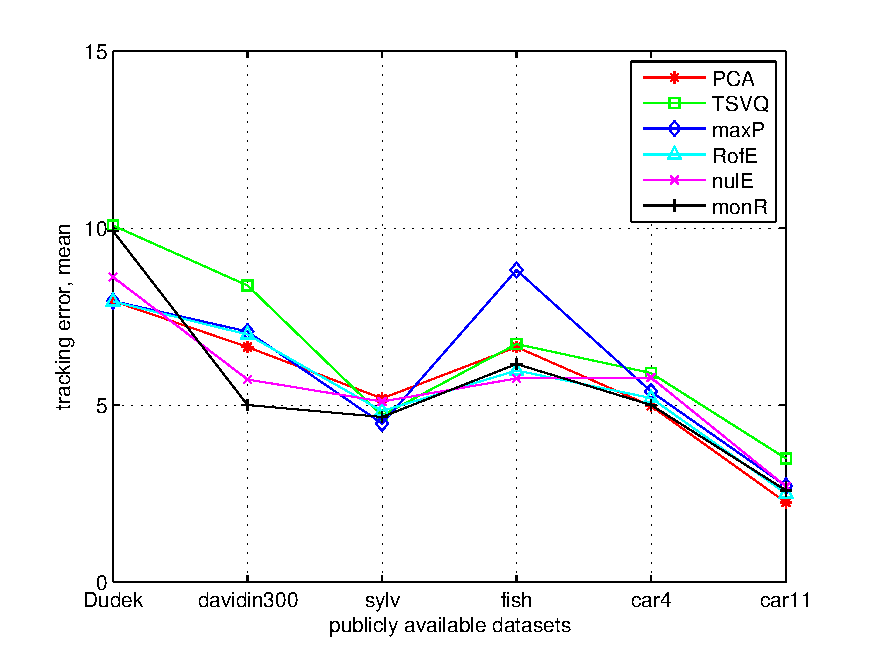
\includegraphics[width=0.47\textwidth]{thesis/results_final_2a_mean.pdf}\label{fig:results_final_2a_mean}}
								\subfigure[\%age of datasets over which best mean tracking error is achieved over all parameters.]{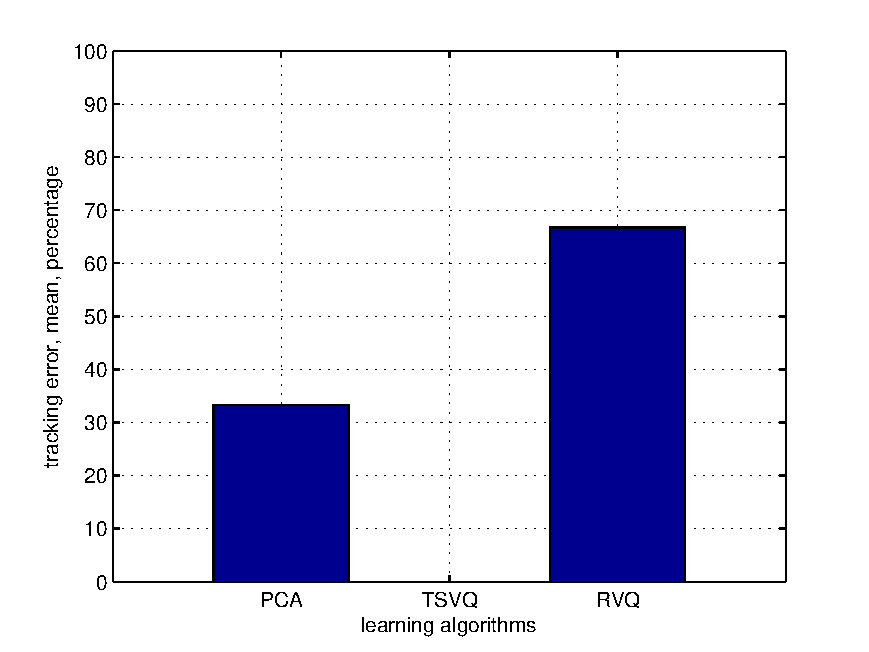
\includegraphics[width=0.47\textwidth]{thesis/results_final_2b_mean_percent.pdf}\label{fig:results_final_2b_mean_percent}}
								\caption{Tracking results (2 of 5), comparison of mean tracking performance.  RVQ performs better over twice as many datasets as PCA.}
								\label{fig:results_final_2_mean}
								\end{figure}


%\begin{enumerate}
%\item \underline{Continually increasing error}.  For Dudek and sylv, the error continues to increase from $Q=8$ to $Q=32$.
%\item \underline{Sharply decreasing, then sharply increasing error}. For davidin300 and fish, the error decreases from $Q=8$ to $Q=16$, and then increases from $Q=16$ to $Q=32$.   The tracking error at $Q=16$ is significantly lower than for $Q=8$ and $Q=32$.
%\item \underline{Mildly decreasing, then mildly increasing error}.  For car4 and car11, like for davidin300 and fish above, the error decreases from $Q=8$ to $Q=16$, and then increases from $Q=16$ to $Q=32$.  However, the drop and rise in error is not as steep.
%\item \underline{Highest error}.  The average error for the Dudek sequence is highest.  This is because this sequence contains more variation than all other sequences including temporary occlusions, expression changes, structured noise, lighting changes and pose changes.  
%\item \underline{Face tracking}.  
%\end{enumerate}

For the Dudek and davidin300 sequences which consist of tracking a face, we look at some related areas in the context of facial processing using PCA, 

\begin{enumerate}
\item \underline{Face reconstruction}.  It has been shown that 40 eigenfaces can be used to reconstruct a face with 3\% error~\cite{1987_JNL_Faces_Sirovich}.
\item \underline{Face recognition}.  Face recognition performance levels off at about 25 principal components, or 45 principal components if the first 3 principal components are dropped~\cite{1997_JNL_EigenVsFisherFaces_Bel}.  The reason for dropping 3 principal components is that~\cite{1992_THE_GeoPhoto_Shashua} showed that for a fixed viewpoint, images of a Lambertian surface\footnote{A Lambertian surface, or informally a matte surface, is a surface that has constant BRDF (bidirectional reflectance distribution function).  BRDF has been explained earlier.} under varying lighting conditions lie in a 3D linear subspace of the high-dimensional image space.
\item \underline{Accounting for lighting changes in face recognition}.  As mentioned above, the first 3 principal components account for lighting changes in faces.  However, these components are unlikely to only account for lighting variation and removing them may result in loss of important information~\cite{1997_JNL_EigenVsFisherFaces_Bel}.
\end{enumerate}

								\begin{figure}[t]
								\centering
								\begin{tabular}{|l|c|c|c|c|c|c|}
\hline
&\textbf{PCA}&\textbf{TSVQ}&\textbf{maxP}&\textbf{RofE}&\textbf{nulE}&\textbf{monR}\\\hline
\textbf{Dudek}&7.81&8.62&7.78&7.11&9.65&11.81\\\hline
\textbf{davidin300}&4.60&12.88&6.84&9.02&7.17&50.00\\\hline
\textbf{sylv}&5.47&4.70&4.00&4.12&4.81&4.31\\\hline
\textbf{fish}&2.17&10.07&11.50&2.96&4.03&2.89\\\hline
\textbf{car4}&4.60&5.11&4.67&4.93&5.28&5.07\\\hline
\textbf{car11}&2.13&2.21&2.17&2.47&2.59&2.47\\\hline
\textbf{ \% best}&66.67&0.00&16.67&16.67&0.00&0.00\\\hline
\end{tabular}

								\subfigure[Tracking error for each algorithm with 16 eigenvectors/code-vectors stored in memory.]{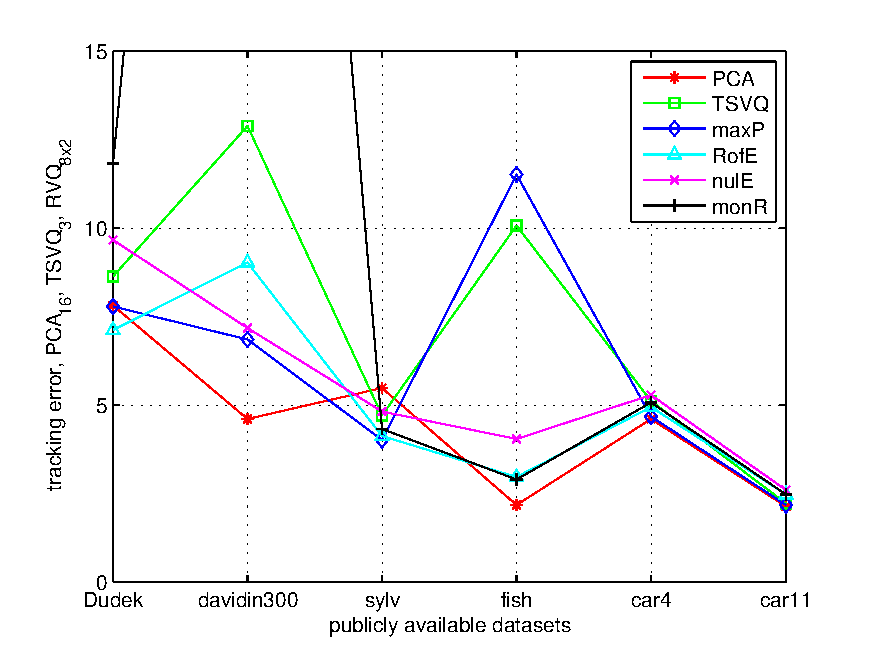
\includegraphics[width=0.47\textwidth]{thesis/results_final_3a_16.pdf}\label{fig:results_final_3a_16}}
								\subfigure[\%age of datasets over which best tracking error is achieved with 16 eigenvectors/code-vectors stored in memory.]{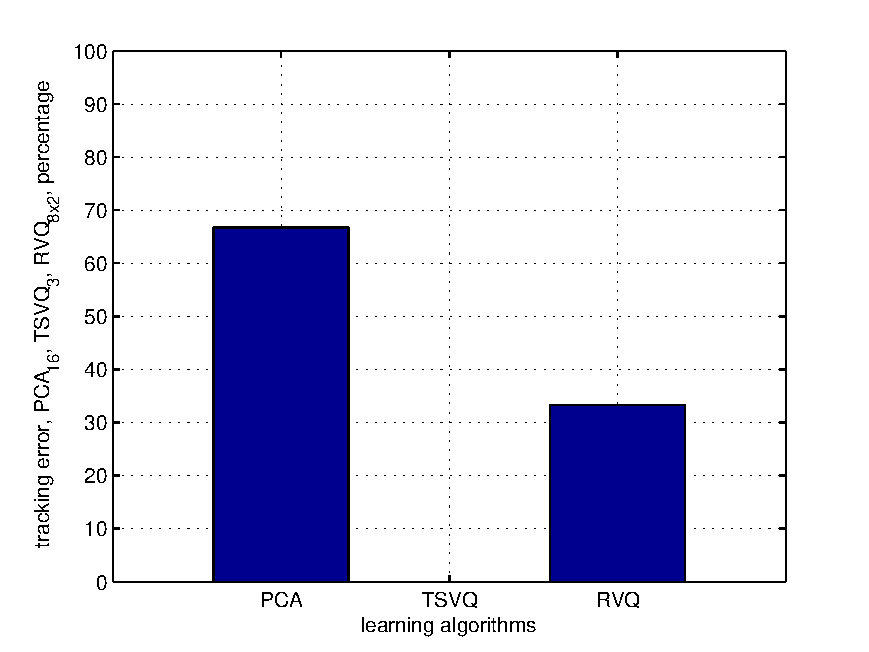
\includegraphics[width=0.47\textwidth]{thesis/results_final_3b_16_percent.pdf}\label{fig:results_final_3b_16_percent}}
								\caption{Tracking results (3 of 5), comparison of tracking performance if 16 eigenvectors/code-vectors are stored in memory.  PCA performs better over twice as many datasets as RVQ.}
								\label{fig:results_final_3_16}
								\end{figure}

Given these observations in related areas of facial processing, we do not remove any principal components.  However, unlike the face recognition case, our tracking performance does not keep increasing till 20 or more eigenvectors.  An important difference in tracking applications however is that face alignment is noisy.  It appears that in the Dudek and davidin300 sequences which have large pose changes, the first few eigenvectors are able to capture the linear dependencies in the slightly shifted faces.  After that, the later eigenvectors explain the residual noise.  This can lead to decreased tracking performance since reconstructions using an eigenspace that partially explains noise will be noisy.  Noisy reconstructions will get inaccurate DFFS (distance-from-feature-space) scores, which in turn will cause incorrect weighting for particle filter candidates in the tracking process.  This will lead to larger tracking error.

								\begin{figure}[t]
								\centering
								\begin{tabular}{|l|c|c|c|c|c|c|}
\hline
&\textbf{PCA}&\textbf{TSVQ}&\textbf{maxP}&\textbf{RofE}&\textbf{nulE}&\textbf{monR}\\\hline
\textbf{Dudek}&8.54&11.87&7.92&8.43&8.19&9.17\\\hline
\textbf{davidin300}&6.93&6.29&4.47&6.21&5.35&5.83\\\hline
\textbf{sylv}&5.72&4.80&4.68&5.54&5.74&4.58\\\hline
\textbf{fish}&7.98&4.59&2.78&12.22&2.48&3.62\\\hline
\textbf{car4}&5.52&6.79&6.38&5.14&5.84&5.18\\\hline
\textbf{car11}&2.39&5.28&2.36&2.33&2.52&2.72\\\hline
\textbf{ \% best}&0.00&0.00&33.33&33.33&16.67&16.67\\\hline
\end{tabular}

								\subfigure[Tracking error for each algorithm with 32 eigenvectors/code-vectors stored in memory.]{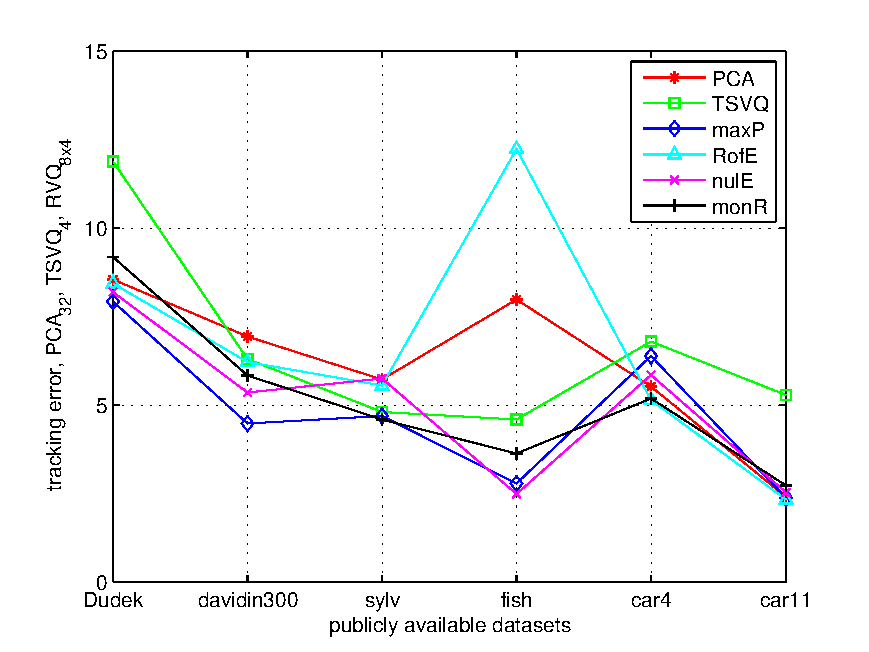
\includegraphics[width=0.47\textwidth]{thesis/results_final_4a_32.pdf}\label{fig:results_final_4a_32}}
								\subfigure[\%age of datasets over which best tracking error is achieved with 32 eigenvectors/code-vectors stored in memory.]{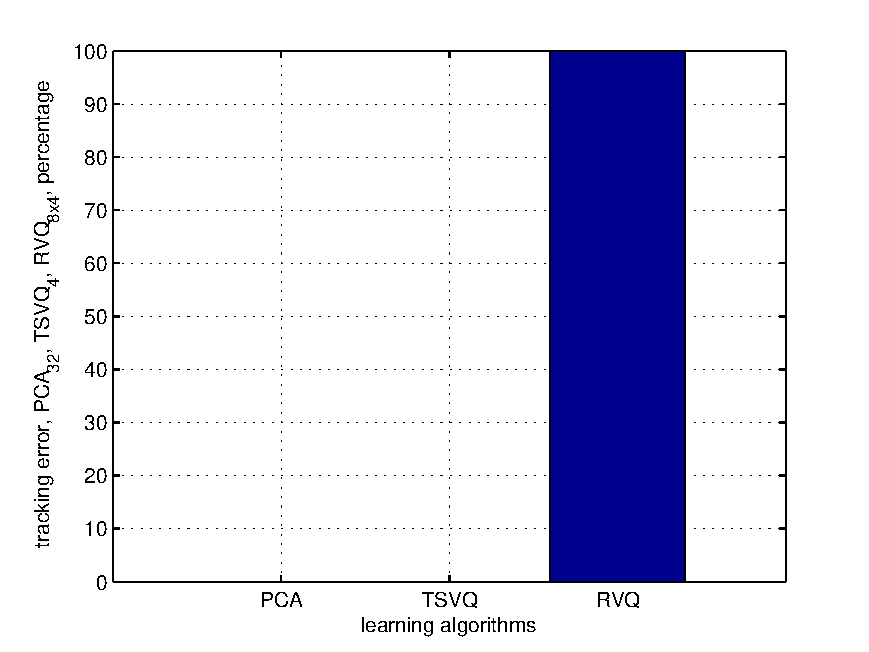
\includegraphics[width=0.47\textwidth]{thesis/results_final_4b_32_percent.pdf}\label{fig:results_final_4b_32_percent}}
								\caption{Tracking results (4 of 5), comparison of tracking performance if 32 eigenvectors/code-vectors are stored in memory.  RVQ performs the best over all datasets.}
								\label{fig:results_final_4_32}
								\end{figure}

Our final tracking results are plotted in 5 figures, Figures~\ref{fig:results_final_1_best}, \ref{fig:results_final_2_mean}, \ref{fig:results_final_3_16}, \ref{fig:results_final_4_32} and~\ref{fig:results_final_5_configs}.  These plots are based entirely on detailed plots in Figures~\ref{fig:results_final_pca_}, \ref{fig:results_final_tsvq}, \ref{fig:results_final_maxP}, \ref{fig:results_final_RofE} \ref{fig:results_final_nulE} and \ref{fig:results_final_monR} in Appendix~\ref{App:tracking_error_plots} for PCA, TSVQ, maxP, RofE, nulE and monR respectively.

We draw several conclusions from these results.  These are given in the next chapter.

								\begin{figure}[h!]
								\centering
	
								\subtable[PCA.]{\begin{tabular}{|c|c|c|c|}
\hline
\textbf{8}&\textbf{16}&\textbf{32}&\textbf{mean}\\\hline
6.15&4.46&6.18&5.60\\\hline
\end{tabular}
}
								\subtable[TSVQ.]{\begin{tabular}{|c|c|c|c|}
\hline
\textbf{3}&\textbf{4}&\textbf{5}&\textbf{mean}\\\hline
7.26&6.60&5.74&6.54\\\hline
\end{tabular}
}
								\subtable[maxP.]{\begin{tabular}{|c|c|c|c|}
\hline
\textbf{8x2}&\textbf{8x4}&\textbf{8x8}&\textbf{mean}\\\hline
6.16&4.76&7.25&6.06\\\hline
\end{tabular}
}
								\subtable[RofE.]{\begin{tabular}{|c|c|c|c|}
\hline
\textbf{8x2}&\textbf{8x4}&\textbf{8x8}&\textbf{mean}\\\hline
5.10&6.64&4.94&5.56\\\hline
\end{tabular}
}
								\subtable[nulE.]{\begin{tabular}{|c|c|c|c|}
\hline
\textbf{8x2}&\textbf{8x4}&\textbf{8x8}&\textbf{mean}\\\hline
5.59&5.02&6.20&5.60\\\hline
\end{tabular}
}
								\subtable[monR.]{\begin{tabular}{|c|c|c|c|}
\hline
\textbf{8x2}&\textbf{8x4}&\textbf{8x8}&\textbf{mean}\\\hline
5.31&5.18&6.19&5.56\\\hline
\end{tabular}
}
								\subtable[maxP, RofE, nulE, monR.]{\begin{tabular}{|c|c|c|}
\hline
\textbf{8x2}&\textbf{8x4}&\textbf{8x8}\\\hline
5.54&5.40&6.15\\\hline
\end{tabular}
}\\
								\subfigure[PCA]{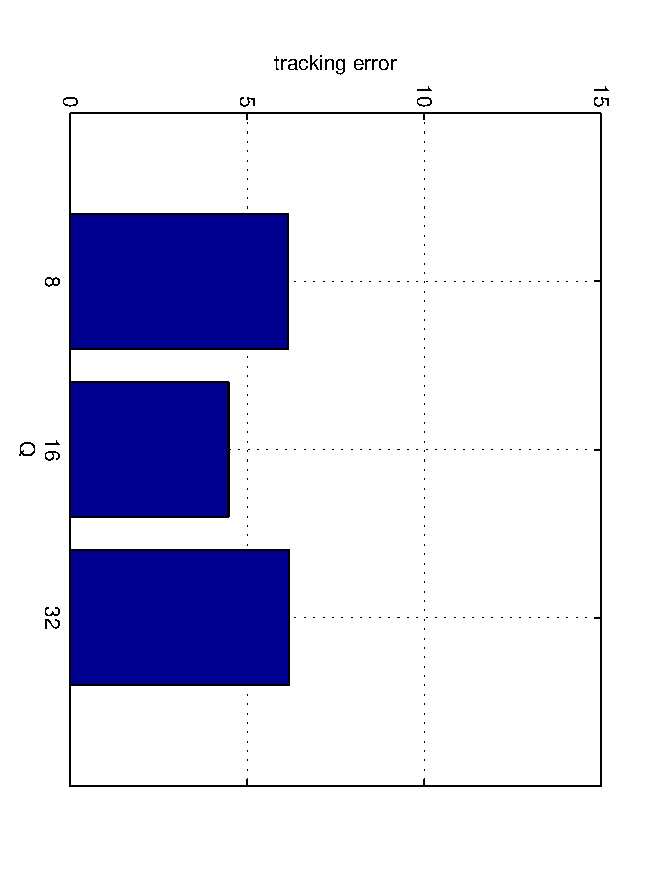
\includegraphics[width=0.225\textwidth, angle=90]{thesis/results_final_5a_pca_.pdf}\label{fig:results_final_5a_pca_}}
								\subfigure[TSVQ.]{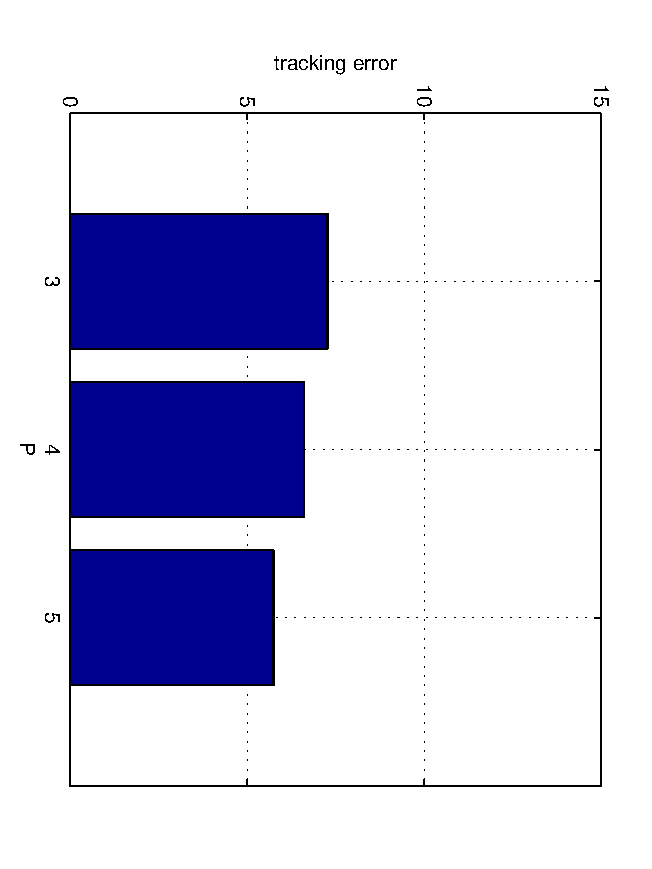
\includegraphics[width=0.225\textwidth, angle=90]{thesis/results_final_5b_tsvq.pdf}\label{fig:results_final_5b}}
								\subfigure[maxP.]{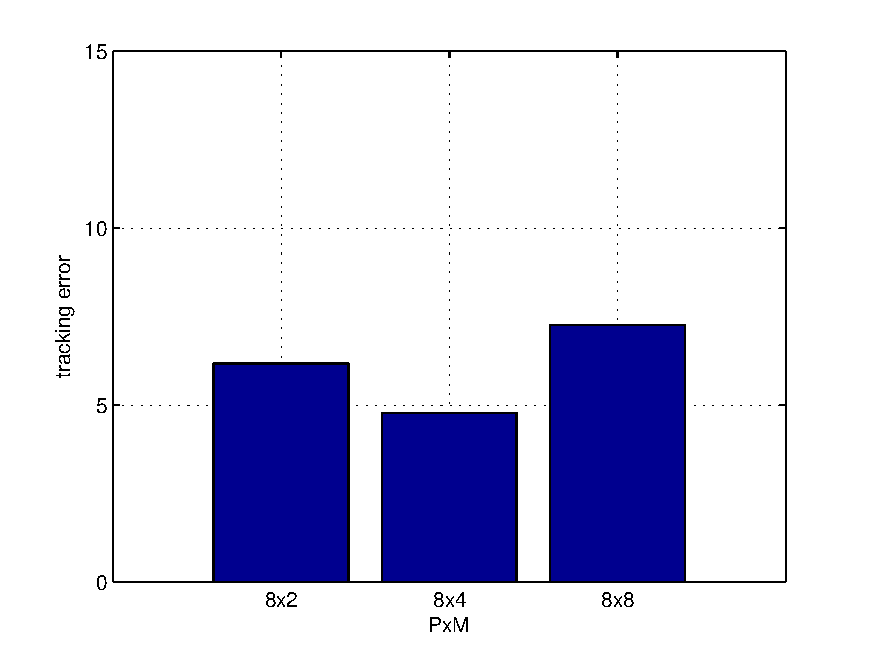
\includegraphics[width=0.3\textwidth]{thesis/results_final_5c_maxP.pdf}\label{fig:results_final_5c}}
								\subfigure[RofE.]{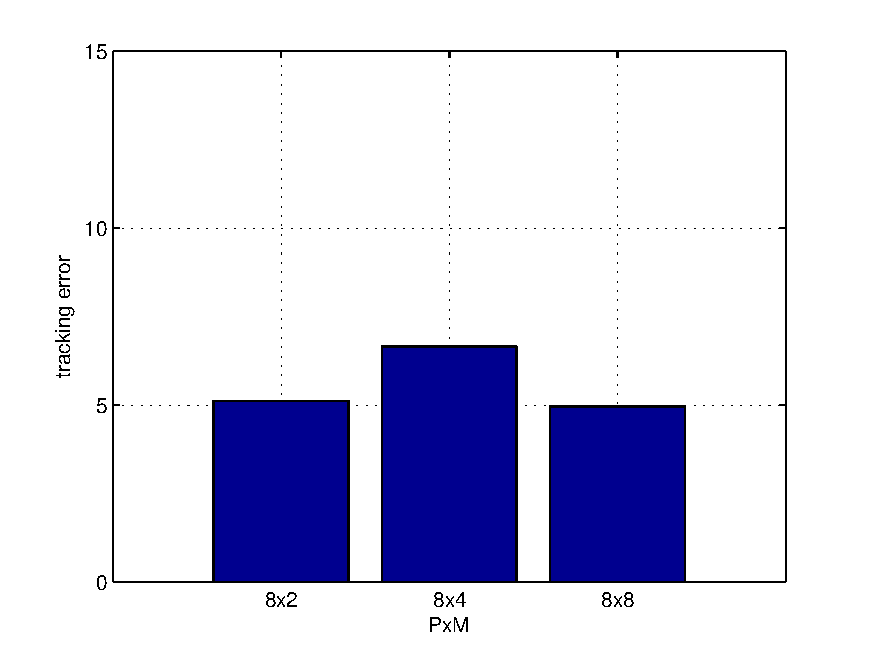
\includegraphics[width=0.3\textwidth]{thesis/results_final_5d_RofE.pdf}\label{fig:results_final_5d}}
								\subfigure[nulE.]{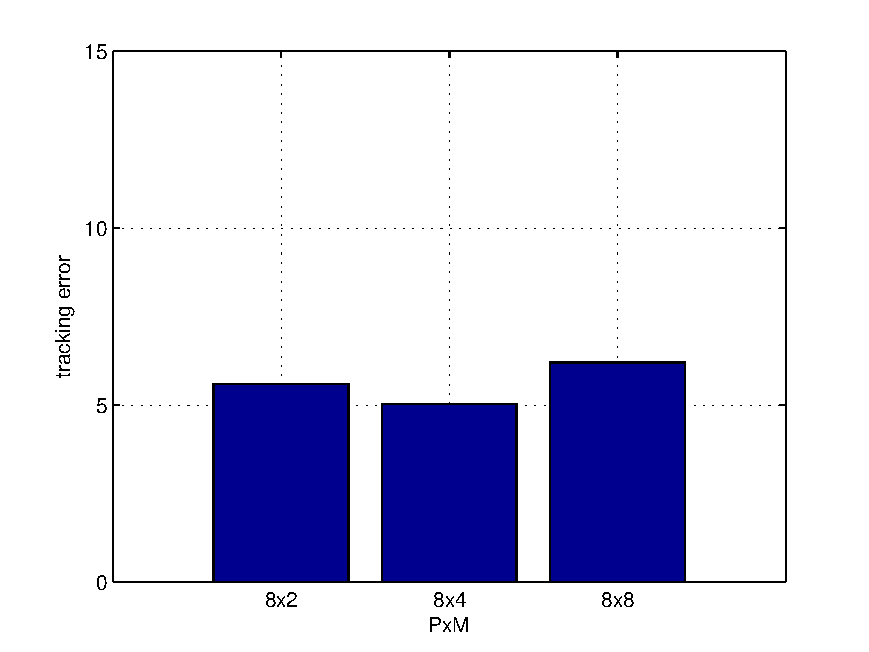
\includegraphics[width=0.3\textwidth]{thesis/results_final_5e_nulE.pdf}\label{fig:results_final_5e}}
							\subfigure[monR.]{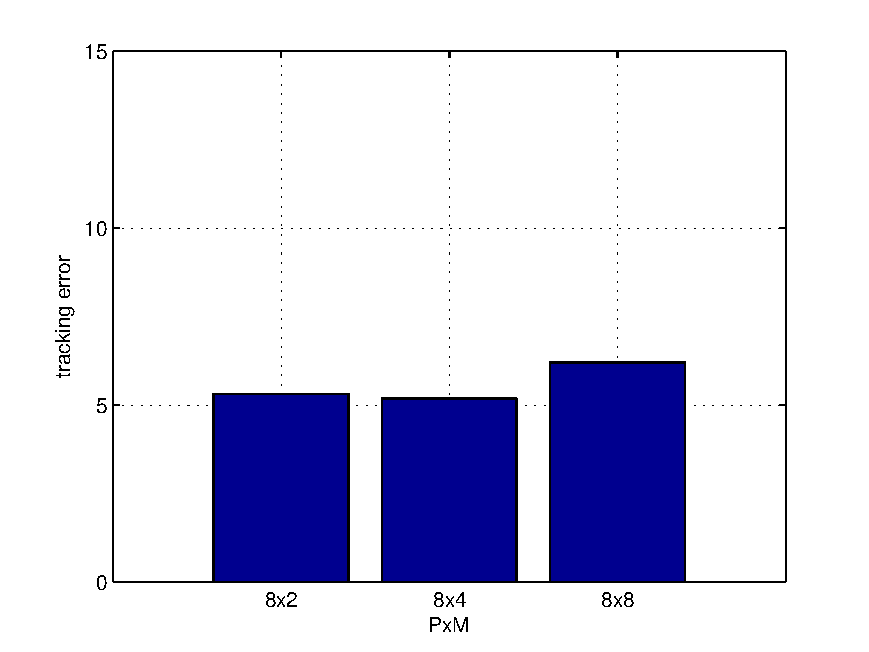
\includegraphics[width=0.3\textwidth]{thesis/results_final_5f_monR.pdf}\label{fig:results_final_5f}}
								\subfigure[maxP, RofE, nulE, monR.]{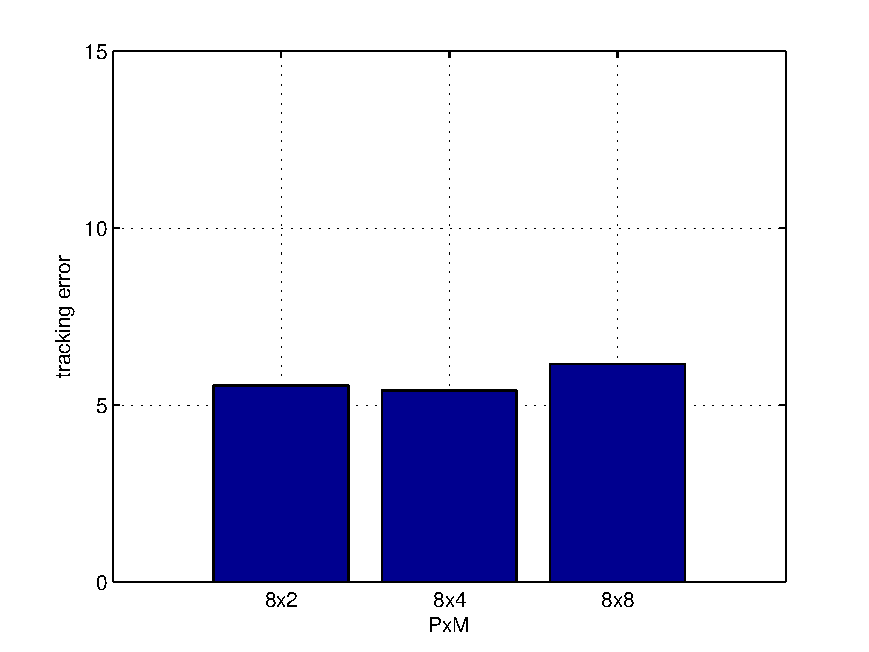
\includegraphics[width=0.3\textwidth]{thesis/results_final_5g_8x2_8x4_8x8.pdf}\label{fig:results_final_5g_8x2_8x4_8x8}}
								\caption{Tracking results (5 of 5), comparison of tracking performance as parameters for each algorithm are varied.  In (d), we see that over all RVQ algorithms, RofE has best mean performance.  In (g) it is clear that the best RVQ configuration is 8x4.}
								\label{fig:results_final_5_configs}
								\end{figure}



We start with Figure~\ref{fig:results_final_1_best}.  In this figure, we plot best possible tracking performance for each algorithm.  For PCA, this means the best possible performance attained for each of the datasets for $Q$=8, 16 and 32.  For TSVQ, best possible performance for each dataset is over $P$=3, 4 and 5.  For maxP, RofE, nulE and monR, best possible performance for each dataset is over 8x2, 8x4 and 8x8.  The reason for plotting performance for each dataset separately is that each dataset represents a different distribution and we would like to gauge performance for each algorithm over the different distributions.  We see that performance for PCA and all 4 RVQ based algorithms is very close while TSVQ tracking error is highest in most cases.  

PCA performs best in the fish, car4 and car11 sequences while RVQ performs best in the remaining three datasets, Dudek, davidin300 and sylv.  TSVQ does not perform best in any sequence.  Note that the performance difference between PCA and RVQ in the car4 and car11 sequences is negligible.  Recall that car4 and car11 are relatively benign datasets with little variation in pose and lighting.  The fish sequence has sudden motion as well as sudden global lighting changes.   Since global lighting change induces linear correlation in the data, it makes sense that PCA does well in this sequence.  The reason is that global illumination moves the illuminated object within the modeled PCA subspace~\cite{1987_JNL_Faces_Sirovich}.  For a VQ based method such as RVQ or TSVQ, several codevectors would have to be dedicated to different lighting conditions to model all possible lighting changes.  

RVQ performs best over the Dudek, davidin300 and sylv sequences.  All 3 of these sequences have moderate lighting changes while Dudek and davidin300 have several forms of noise as discussed earlier.  For Dudek, RofE does best.  The reason is that in the presence of uncertainties, RofE holds tight to what has already been modeled and is resistant to accepting sudden changes in the underlying distribution.  It is therefore better able to handle blur and other forms of noise that did not exist in the training data.  On the other extreme is monR which greedily attempts to minimize reconstruction error.  Out of all RVQ methods, this method performs worse, but even then, not by much.  Second best performance is for maxP which is again not a greedy method.  Third best performance is for nulE which is also a greedy method but less so than monR.

We now turn to Figure~\ref{fig:results_final_2_mean}.  In this figure, mean performance over all configurations is shown.  It may be noted that monR loses track in one instance.  That instance is not factored into the means since it is not clear how penalize a lost track when performing mean computations.  Here, we see that RVQ performs best 66.7\% of the time.  This time, in addition to Dudek, davindin300 and sylv, RVQ performs better than PCA in the fish sequence as well.  The reason for this is that PCA is unable to track the fish sequence well when it has too few, i.e., 8 eigenvectors or when it has too many, i.e., 32 eigenvectors.  In the 8 eigenvector case, the subspace does not have enough dimensions to model lighting changes well.  Even though it has been shown, as mentioned earlier, that only 3 eigenvectors are needed to model lighting changes~\cite{1987_JNL_Faces_Sirovich}, in practice this does not hold due to shadowing and specularities~\cite{1997_JNL_EigenVsFisherFaces_Bel}.  For too many eigenvectors, over-fitting is an issue as mentioned in an earlier report.  For $Q=16$, PCA performs best and that is why it had best possible performance.  However, when it comes to means, all 4 RVQ configurations are able to outperform PCA in mean performance.

In Figures~\ref{fig:results_final_3_16} and~\ref{fig:results_final_4_32}, we hold the number of eigenvectors for PCA or codevectors for TSVQ and RVQ constant at 16 and 32 respectively\footnote{This is 15 and 31 actually for TSVQ but we ignore this slight difference.}.  In these figures, we see that PCA outperforms RVQ for 16 vectors but RVQ completely outperforms PCA for 32 vectors.  For a given memory cost, and therefore for a given rate, RVQ overall outperforms PCA.  

Finally, in Figure~\ref{fig:results_final_5_configs}, we plot tracking performance for each algoritm separately for its different configurations.  For 3 configurations per algorithm, $Q$=8, 16, 32 for PCA, $P$=3, 4, 5 for TSVQ and $PxM$ = 8x2, 8x4, 8x8 for RVQ, there are 4 possible outcomes listed below.  Of these, the first 3 are to be expected.  The fourth however requires further scrutiny.

\begin{enumerate}
\item \underline{Monotonically increasing error.}  This would mean that the degrees of freedom (DoF) in the learning algorithm, such as PCA, TSVQ or RVQ, model the underlying distribution well with low DoFs and adding DoFs is leading to over-generalization.  We do not see this performance in any case since we start with low DoFs.  We got an initial estimate of how many DoFs to use using our experiments on appearance modeling that have mentioned in a previous report.
\item \underline{Monotonically decreasing error.}  This happens for TSVQ.  This means that adding more stages to TSVQ may increase performance.  In our case, we use 3, 4 and 5 stages to keep the DoFs in TSVQ close to the DoFs for RVQ and PCA.
\item \underline{Decreasing error followed by increasing error.}  We see this performance for PCA, maxP, nulE and monR.  This is a sign that the correct number of DoFs were chosen and that when error is minimum, the algorithm now has enough capacity to model the underlying distribution, but without over-fitting.
\item \underline{Increasing error followed by decreasing error.}  We see this in one case, RofE, and in some cases in TSVQ in Figure~\ref{fig:results_final_tsvq}.  To see this, consider the example of $K$=2, 4 and 8 code-vectors in $\mathbb{R}$ uniformly spaced on the inteval [0,7].  For $K$=2, the code-vectors are 2.33 and 4.66.  For the $K$=4 case, the code-vectors are 1.4, 2.8, 4.2 and 5.6.  For the $K$=8 case, the code-vectors are $\{0, 1, 2, 3, \ldots, 7\}$.  In regions around 2.33 and 4.6, there are certain contiguous regions where the reconstruction error is greatest for $K$=4.  This shows that although in general, one would not expect reconstruction error, and therefore tracking error to be lowest for an intermediate number of code-vectors $K$, it is possible for a test vector to score highest error for an intermediate $K$.  If this occurs at a point in the tracking process where the target is moving quickly for instance, then a wrong decision can cause tracking error to increase.  In certain cases, it may not be possible to recover from this wrong decision.  See Figures~\ref{fig:results_TSVQ_Dudek_errors}, \ref{fig:results_TSVQ_Dudek_FN10} and \ref{fig:results_TSVQ_Dudek_FN457} in Appendix~\ref{App:TSVQ_Dudek_example} for an example of such a scenario for TSVQ tracking.


\end{enumerate}

%
%For PCA, on average, $Q=16$ produces the lowest tracking error.  On average, the tracking error decreases from $Q=8$ to $Q=16$, and then increases from $Q=16$ to $Q=32$.  It appears that the number of eigenvectors required to capture the linear correlation in these datasets is between 16 and 32, but closer to 16.   







%\begin{table}[h!]
%\centering
%\begin{tabular}{|l|c|c|c|}
\hline
&\textbf{PCA}&\textbf{TSVQ}&\textbf{RVQ}\\\hline
\textbf{Dudek}&7.44&8.62&6.68\\\hline
\textbf{davidin300}&4.60&5.93&4.29\\\hline
\textbf{sylv}&4.34&4.61&4.19\\\hline
\textbf{fish}&2.17&4.59&2.60\\\hline
\textbf{car4}&4.60&5.11&4.72\\\hline
\textbf{car11}&2.13&2.21&2.00\\\hline
\textbf{mean}&4.21&5.18&4.08\\\hline
\end{tabular}

%\caption{Comparison of best possible tracking error between PCA, RVQ and TSVQ over all algorithm parameters for 6 publicly available challenging datasets, Dudek, davidin300, sylv, fish, car4 and car11.  The table shows that RVQ produces the best results for 4 of the 6 datasets.  Overall tracking error is least for RVQ followed by PCA, and then followed by TSVQ.}
%\end{table}
%
%\begin{table}[h!]
%\centering
%\input{thesis/tables_comparison_DOF_16}
%\caption{Comparison of tracking results using the same DoF, 16 eigenvectors for PCA, 8x2 RVQ and 3x2 TSVQ (15 DOF for TSVQ, 8 terminal code-vectors and 7 stage code-vectors).  RVQ has best overall tracking performance.}
%\end{table}
%
%\begin{table}[h!]
%\centering
%\input{thesis/tables_comparison_DOF_32.tex}
%\caption{Comparison of tracking results using the same DoF, 32 eigenvectors for PCA, 8x4 RVQ and 4x2 TSVQ (31 DOF for TSVQ, 16 terminal code-vectors and 15 stage code-vectors).  RVQ has best tracking performance every time, and therefore also best overall performance.}
%\end{table}


For the interested reader, the appendix contains detailed results for tracking errors for all 6 datasets, for all RVQ types (maxQ, RofE, nulE, monR), over several RVQ configurations (8x2, 8x4, 8x8, 8x12, 8x16).  Also, detailed graphical results for all 6 datasets, for all RVQ types, for the 8x4 configuration are also presented.


%\end{Body}
%%##############################################################################################################
%\begin{EndMatter}
%\references 				%generates the bibliography page
%\end{EndMatter}
%\end{document}
%%##############################################################################################################
%








